
\clearpage
\subsection{Entwurf 0061}\label{sb:0061}
\noindent\textbf{Urteil: }Zulässig (bereinigt), Rang 1 von 7; kleinste Reserve 30 \% (Stahl σ99).\par\smallskip
\begin{minipage}[t]{0.46\linewidth}\small\begin{tabular}[t]{@{}lr@{}}\toprule\multicolumn{2}{@{}l}{\textbf{Stellgrößen}}\\\midrule
Abstand Spule–Plasma & \num{0.204} \\
Spulen gesamt & 24 \\
Spulen je halbe Periode & \num{6} \\
Länge je Spule & \num{4.58} \\
Kraftziel & \num{0.010} \\
Wand innen & \num{0.10} \\
Seitenwand & \num{0.30} \\
Außenwand min. & \num{0.52} \\
Außenwand Zusatz & \num{0.26} \\
Verbindersteifigkeit & \num{93} \\
Verbinder je Paar & \num{10} \\
Lagerradius & \num{3.23} \\
\bottomrule\end{tabular}\end{minipage}\hfill
\begin{minipage}[t]{0.5\linewidth}\small\begin{tabular}[t]{@{}lr@{}}\toprule\multicolumn{2}{@{}l}{\textbf{Ergebnisse}}\\\midrule
$\sigma_{99}$ Stahl & \num{351} MPa \\
größtes Element & \num{725} MPa \\
$P_m$ max. / 99 \% & \num{522} / \num{379} MPa \\
$P_m+P_b$ max. & \num{938} MPa \\
Verbinder σ99 & \num{191} MPa \\
Verformung max. & \num{18} mm \\
Dehnung Wickelpaket & \num{0.17} \% \\
Strom je Spule & \num{14.7} MA \\
Feld am Leiter & \num{15.6} T \\
Auslastung / Marge & \num{30} \% / \num{24} K \\
Feldfehler $B\cdot n$ & \num{1.49} ‰ \\
Freiraum Plasma–Gehäuse & \num{1.62} m \\
Kernheizung / Fluenz & \num{10} W/m³ / 8.0e16 \\
Stahl Gehäuse + Verbinder & \num{9.5} + \num{9.9} kt \\
Verbinder gebaut & 236 \\
\bottomrule\end{tabular}\end{minipage}\par\medskip
\noindent\textit{Netzstudie ($\sigma_{99}$/max. in MPa): }doe1: 351/725; 1,5× Stationen: 556/6553; Wand 3 Zellen: 346/861.\par\smallskip
\begin{figure}[H]\centering
\begin{minipage}[t]{0.49\linewidth}\centering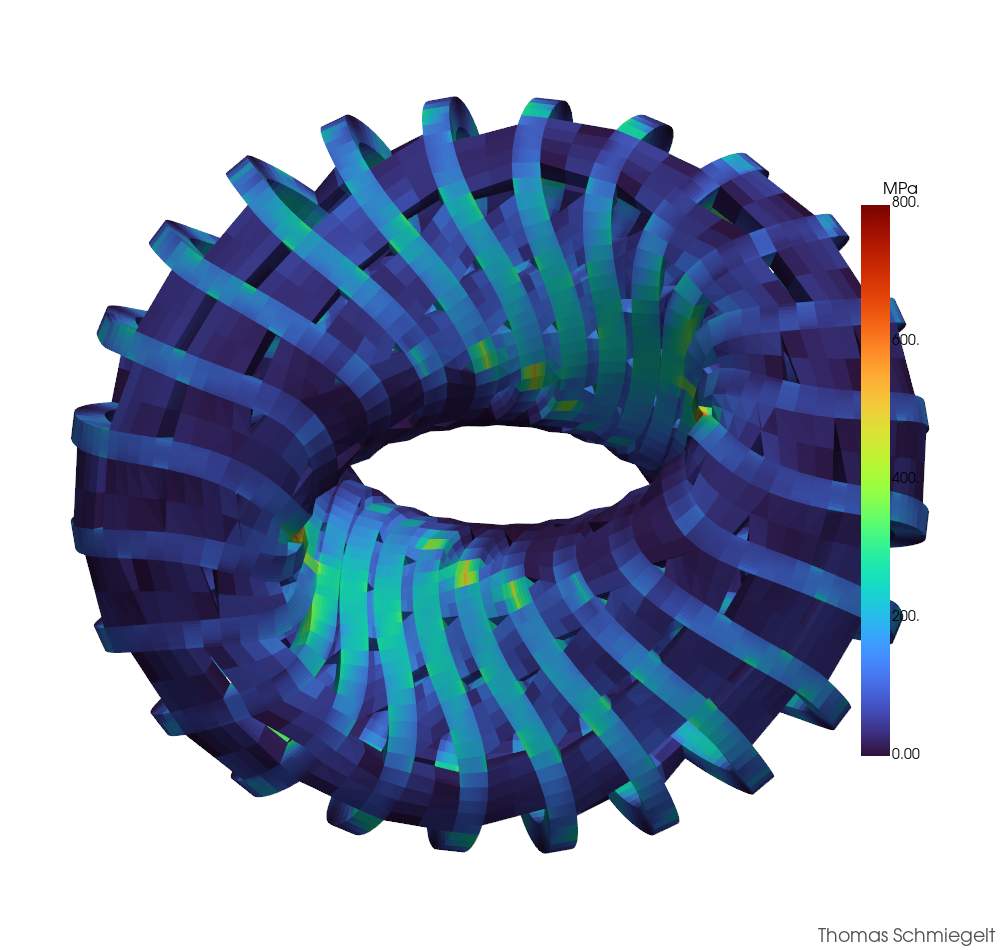
\includegraphics[width=\linewidth]{bilder/spannung_0061.png}\\\footnotesize Vergleichsspannung im Stahl (Draufsicht, 0–800 MPa)\end{minipage}\hfill
\begin{minipage}[t]{0.49\linewidth}\centering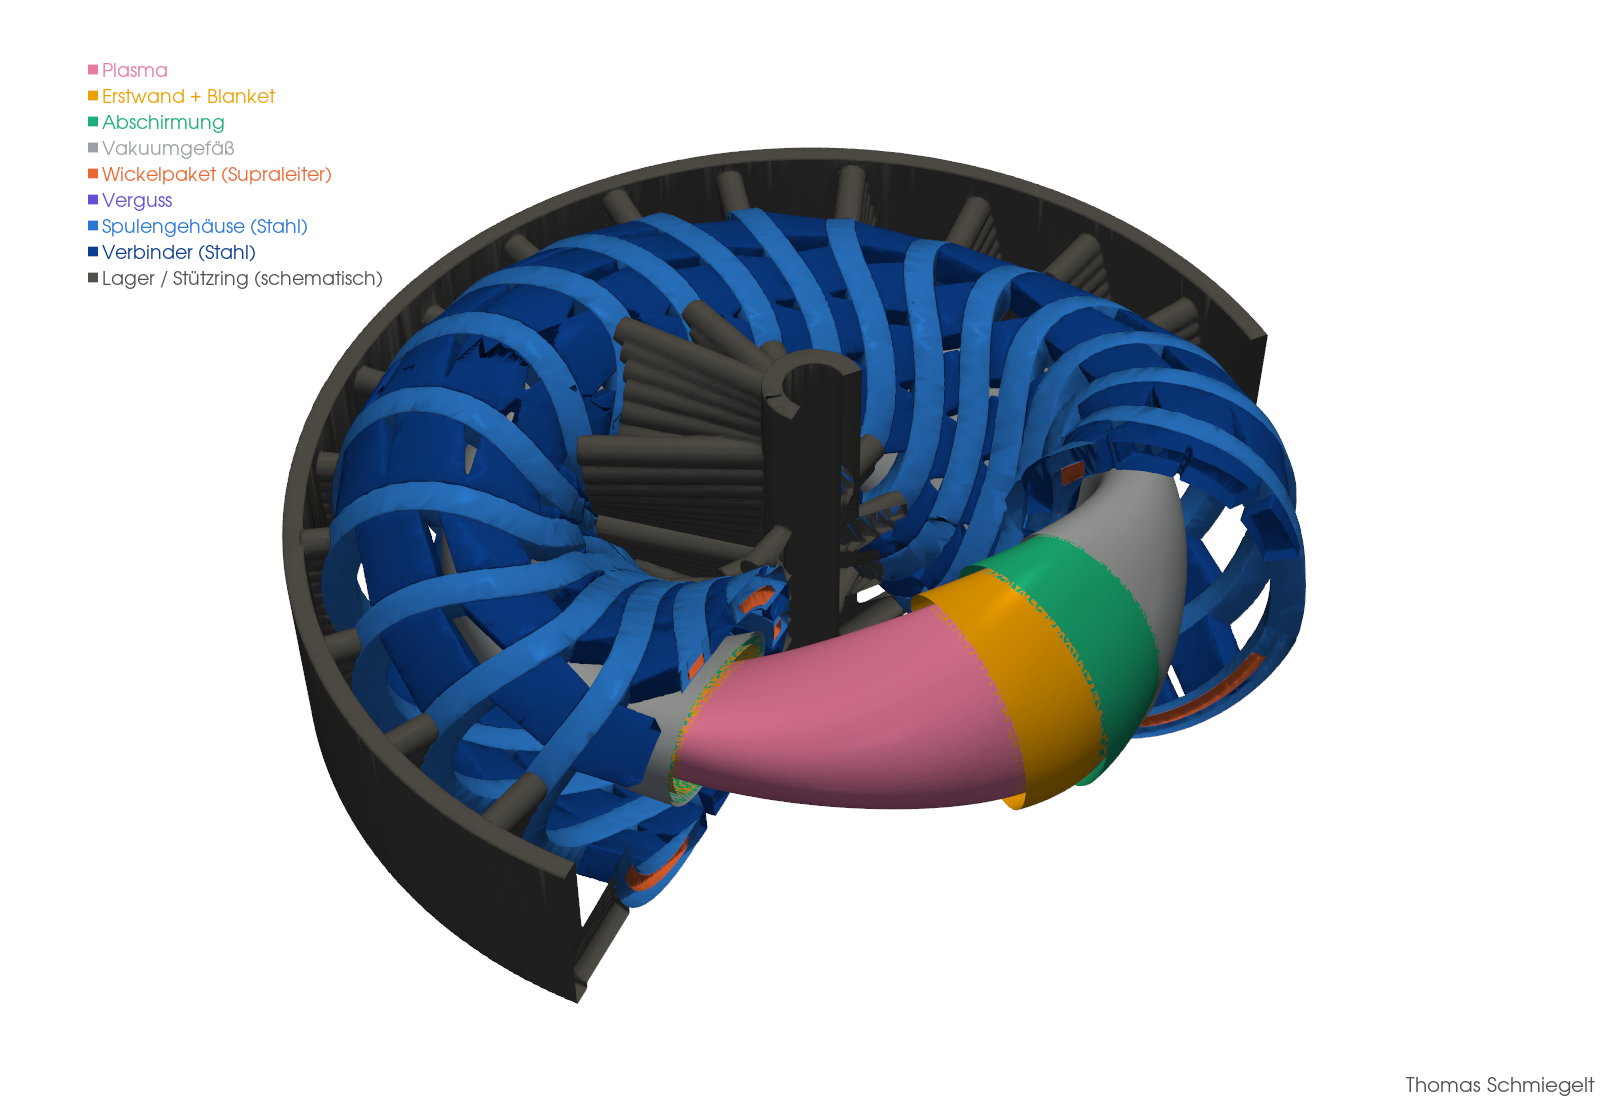
\includegraphics[width=\linewidth]{bilder/modell3d_0061_schnitt.png}\\\footnotesize PicoGK-Modell, Treppenschnitt\end{minipage}\hfill
\caption{Entwurf 0061}\end{figure}
\clearpage
\subsection{Entwurf 0169}\label{sb:0169}
\noindent\textbf{Urteil: }Zulässig (bereinigt), Rang 2 von 7; kleinste Reserve 29 \% (Platz Package).\par\smallskip
\begin{minipage}[t]{0.46\linewidth}\small\begin{tabular}[t]{@{}lr@{}}\toprule\multicolumn{2}{@{}l}{\textbf{Stellgrößen}}\\\midrule
Abstand Spule–Plasma & \num{0.197} \\
Spulen gesamt & 24 \\
Spulen je halbe Periode & \num{6} \\
Länge je Spule & \num{4.87} \\
Kraftziel & \num{0.023} \\
Wand innen & \num{0.27} \\
Seitenwand & \num{0.34} \\
Außenwand min. & \num{0.67} \\
Außenwand Zusatz & \num{0.25} \\
Verbindersteifigkeit & \num{183} \\
Verbinder je Paar & \num{13} \\
Lagerradius & \num{3.29} \\
\bottomrule\end{tabular}\end{minipage}\hfill
\begin{minipage}[t]{0.5\linewidth}\small\begin{tabular}[t]{@{}lr@{}}\toprule\multicolumn{2}{@{}l}{\textbf{Ergebnisse}}\\\midrule
$\sigma_{99}$ Stahl & \num{308} MPa \\
größtes Element & \num{717} MPa \\
$P_m$ max. / 99 \% & \num{626} / \num{333} MPa \\
$P_m+P_b$ max. & \num{817} MPa \\
Verbinder σ99 & \num{192} MPa \\
Verformung max. & \num{19} mm \\
Dehnung Wickelpaket & \num{0.15} \% \\
Strom je Spule & \num{14.7} MA \\
Feld am Leiter & \num{15.5} T \\
Auslastung / Marge & \num{30} \% / \num{24} K \\
Feldfehler $B\cdot n$ & \num{2.13} ‰ \\
Freiraum Plasma–Gehäuse & \num{1.39} m \\
Kernheizung / Fluenz & \num{103} W/m³ / 8.5e17 \\
Stahl Gehäuse + Verbinder & \num{12.8} + \num{15.2} kt \\
Verbinder gebaut & 292 \\
\bottomrule\end{tabular}\end{minipage}\par\medskip
\noindent\textit{Netzstudie ($\sigma_{99}$/max. in MPa): }doe1: 219/421; Standard: 308/717; 1,5× Stationen: 319/1262; Wand 3 Zellen: 308/794.\par\smallskip
\begin{figure}[H]\centering
\begin{minipage}[t]{0.49\linewidth}\centering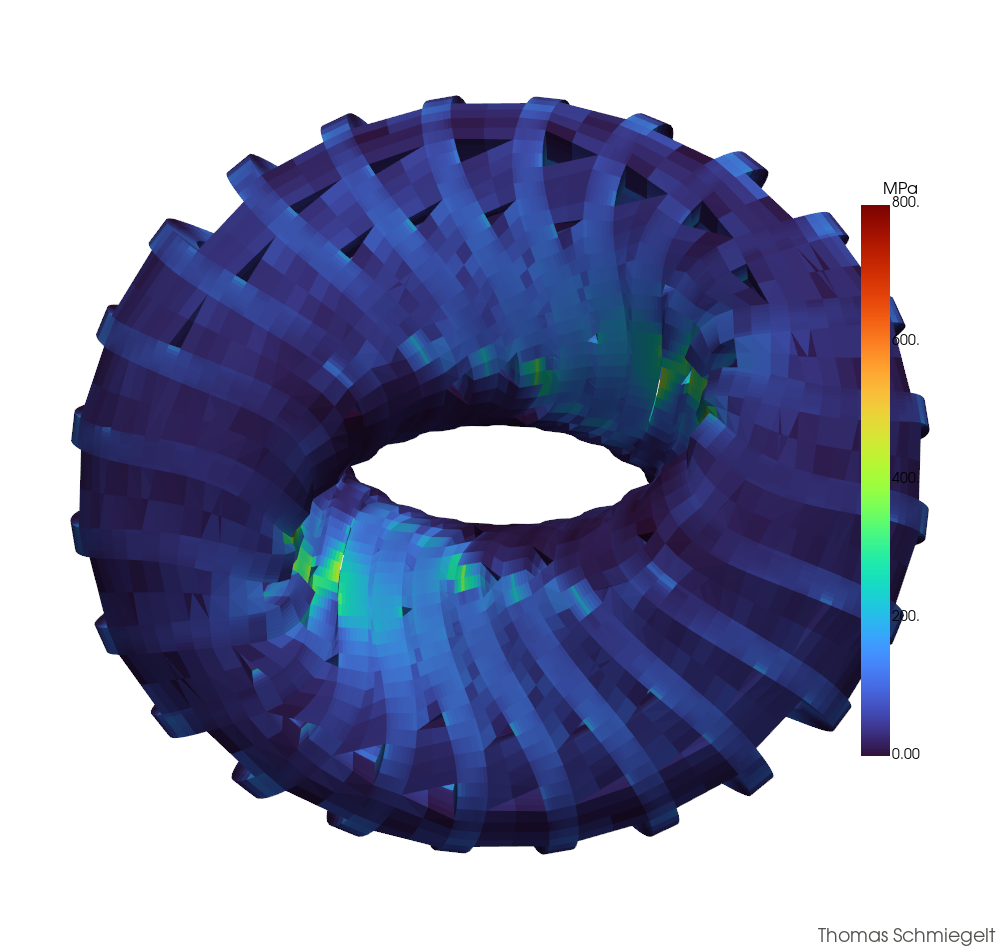
\includegraphics[width=\linewidth]{bilder/spannung_0169.png}\\\footnotesize Vergleichsspannung im Stahl (Draufsicht, 0–800 MPa)\end{minipage}\hfill
\begin{minipage}[t]{0.49\linewidth}\centering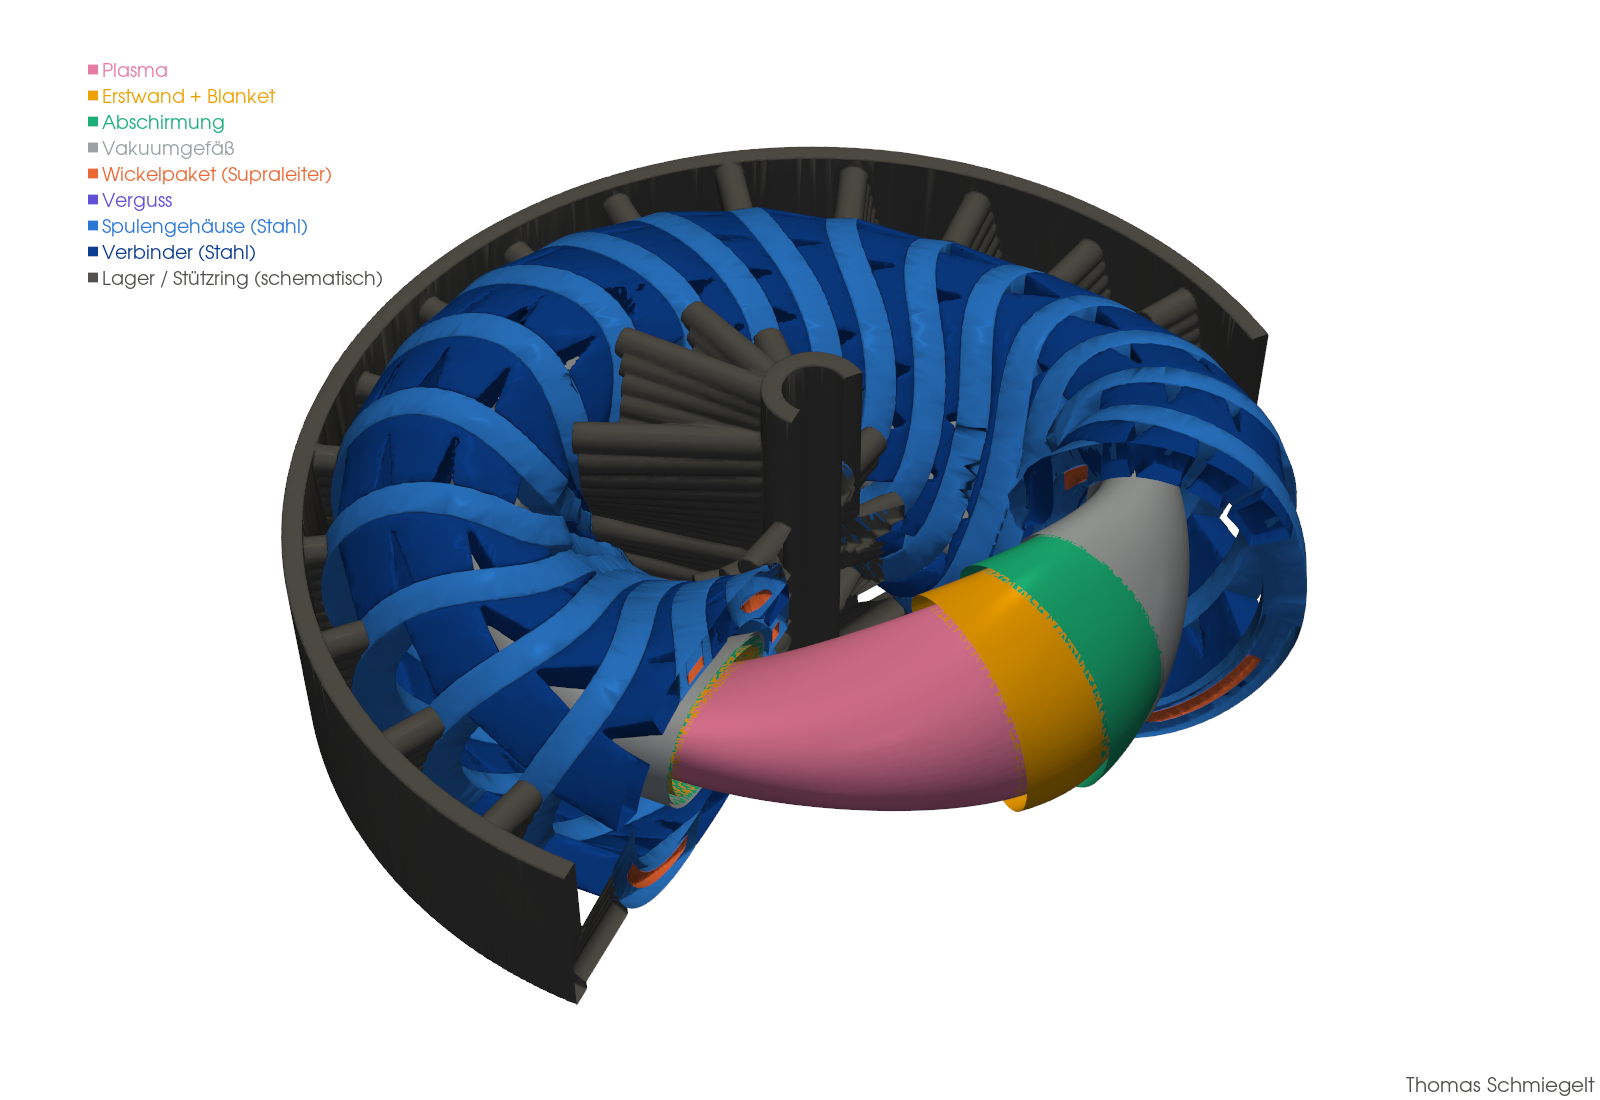
\includegraphics[width=\linewidth]{bilder/modell3d_0169_schnitt.png}\\\footnotesize PicoGK-Modell, Treppenschnitt\end{minipage}\hfill
\caption{Entwurf 0169}\end{figure}
\clearpage
\subsection{Entwurf 0093}\label{sb:0093}
\noindent\textbf{Urteil: }Zulässig (bereinigt), Rang 3 von 7; kleinste Reserve 27 \% (Platz Package).\par\smallskip
\begin{minipage}[t]{0.46\linewidth}\small\begin{tabular}[t]{@{}lr@{}}\toprule\multicolumn{2}{@{}l}{\textbf{Stellgrößen}}\\\midrule
Abstand Spule–Plasma & \num{0.206} \\
Spulen gesamt & 24 \\
Spulen je halbe Periode & \num{6} \\
Länge je Spule & \num{4.14} \\
Kraftziel & \num{0.010} \\
Wand innen & \num{0.38} \\
Seitenwand & \num{0.38} \\
Außenwand min. & \num{0.73} \\
Außenwand Zusatz & \num{0.38} \\
Verbindersteifigkeit & \num{64} \\
Verbinder je Paar & \num{8} \\
Lagerradius & \num{3.49} \\
\bottomrule\end{tabular}\end{minipage}\hfill
\begin{minipage}[t]{0.5\linewidth}\small\begin{tabular}[t]{@{}lr@{}}\toprule\multicolumn{2}{@{}l}{\textbf{Ergebnisse}}\\\midrule
$\sigma_{99}$ Stahl & \num{283} MPa \\
größtes Element & \num{1190} MPa \\
$P_m$ max. / 99 \% & \num{1147} / \num{340} MPa \\
$P_m+P_b$ max. & \num{1233} MPa \\
Verbinder σ99 & \num{154} MPa \\
Verformung max. & \num{20} mm \\
Dehnung Wickelpaket & \num{0.16} \% \\
Strom je Spule & \num{14.7} MA \\
Feld am Leiter & \num{15.7} T \\
Auslastung / Marge & \num{30} \% / \num{24} K \\
Feldfehler $B\cdot n$ & \num{1.45} ‰ \\
Freiraum Plasma–Gehäuse & \num{1.37} m \\
Kernheizung / Fluenz & \num{117} W/m³ / 9.8e17 \\
Stahl Gehäuse + Verbinder & \num{16.5} + \num{11.6} kt \\
Verbinder gebaut & 190 \\
\bottomrule\end{tabular}\end{minipage}\par\medskip
\noindent\textit{Netzstudie ($\sigma_{99}$/max. in MPa): }doe1: 283/1190; 1,5× Stationen: 410/2343; Wand 3 Zellen: 280/1432.\par\smallskip
\begin{figure}[H]\centering
\begin{minipage}[t]{0.49\linewidth}\centering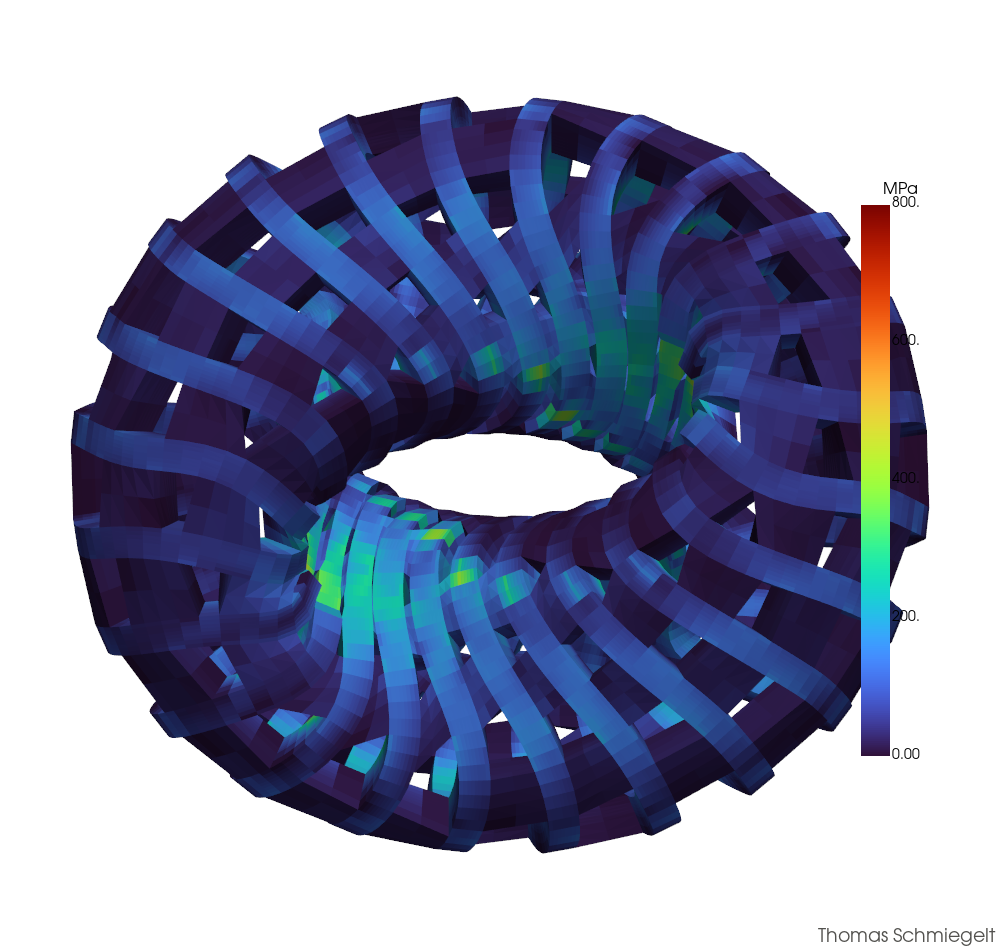
\includegraphics[width=\linewidth]{bilder/spannung_0093.png}\\\footnotesize Vergleichsspannung im Stahl (Draufsicht, 0–800 MPa)\end{minipage}\hfill
\begin{minipage}[t]{0.49\linewidth}\centering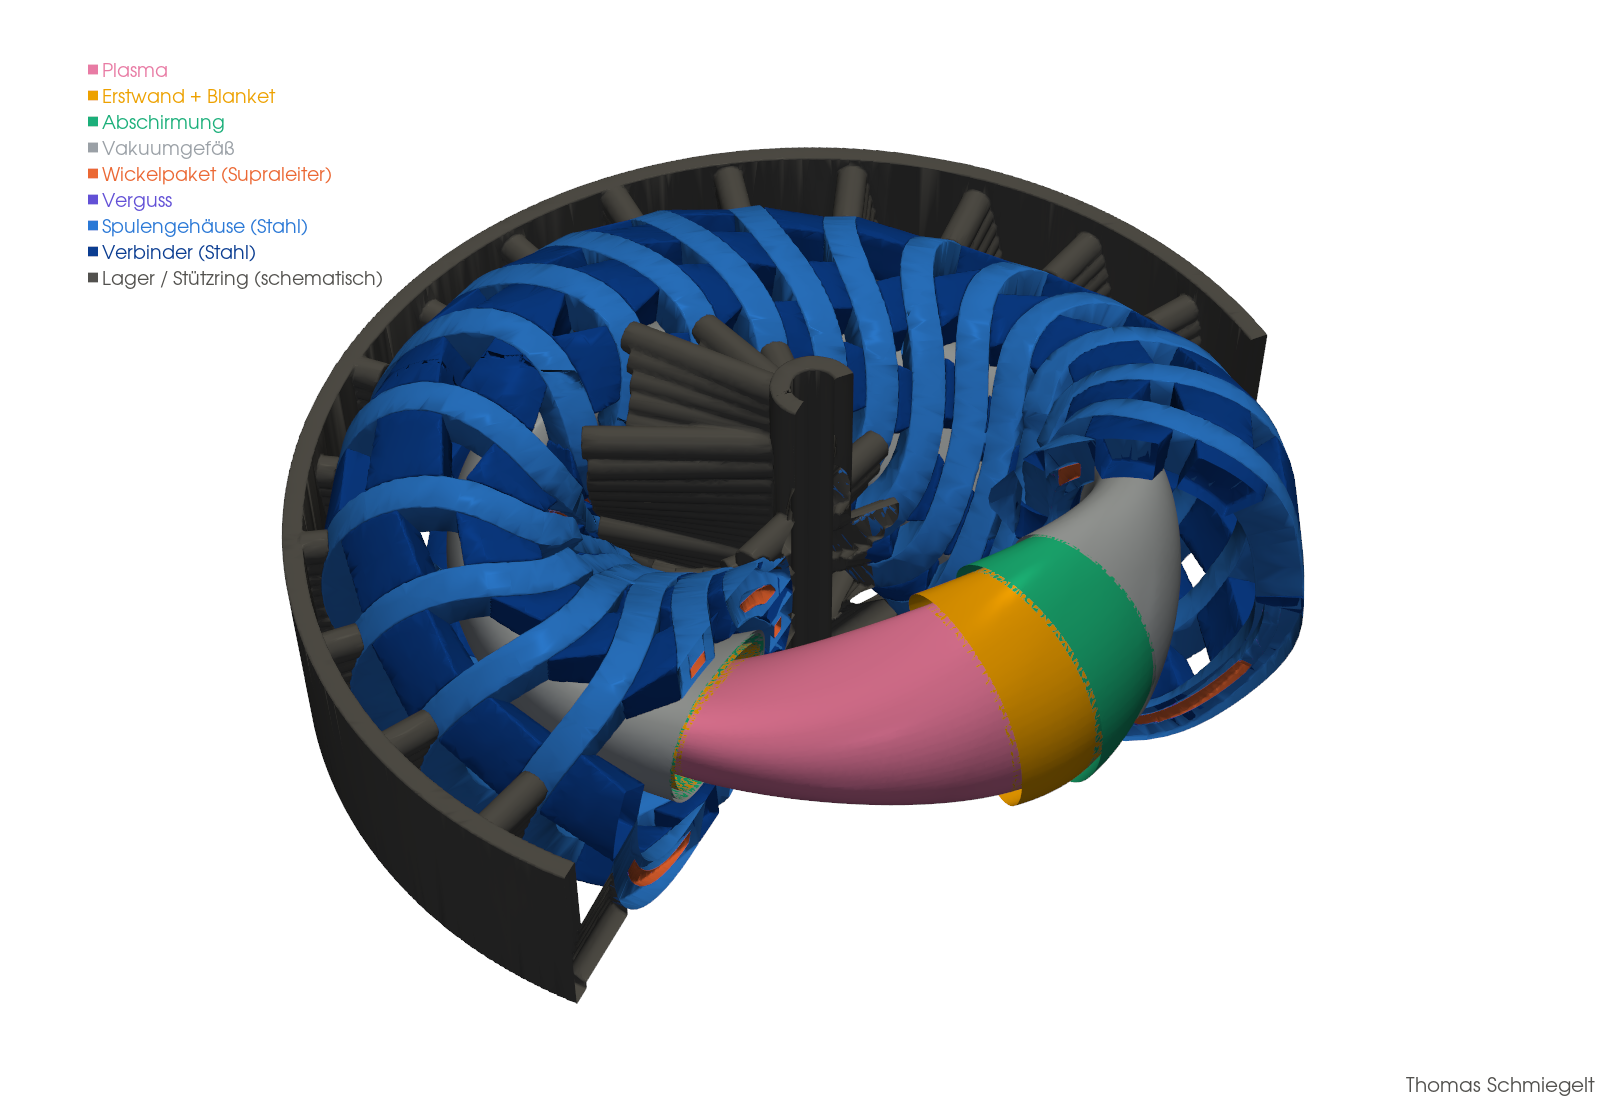
\includegraphics[width=\linewidth]{bilder/modell3d_0093_schnitt.png}\\\footnotesize PicoGK-Modell, Treppenschnitt\end{minipage}\hfill
\caption{Entwurf 0093}\end{figure}
\clearpage
\subsection{Entwurf 0008}\label{sb:0008}
\noindent\textbf{Urteil: }Zulässig (bereinigt), Rang 4 von 7; kleinste Reserve 27 \% (Feldfehler B·n).\par\smallskip
\begin{minipage}[t]{0.46\linewidth}\small\begin{tabular}[t]{@{}lr@{}}\toprule\multicolumn{2}{@{}l}{\textbf{Stellgrößen}}\\\midrule
Abstand Spule–Plasma & \num{0.211} \\
Spulen gesamt & 24 \\
Spulen je halbe Periode & \num{6} \\
Länge je Spule & \num{3.66} \\
Kraftziel & \num{0.030} \\
Wand innen & \num{0.32} \\
Seitenwand & \num{0.31} \\
Außenwand min. & \num{0.72} \\
Außenwand Zusatz & \num{0.17} \\
Verbindersteifigkeit & \num{142} \\
Verbinder je Paar & \num{11} \\
Lagerradius & \num{2.80} \\
\bottomrule\end{tabular}\end{minipage}\hfill
\begin{minipage}[t]{0.5\linewidth}\small\begin{tabular}[t]{@{}lr@{}}\toprule\multicolumn{2}{@{}l}{\textbf{Ergebnisse}}\\\midrule
$\sigma_{99}$ Stahl & \num{305} MPa \\
größtes Element & \num{1695} MPa \\
$P_m$ max. / 99 \% & \num{1687} / \num{344} MPa \\
$P_m+P_b$ max. & \num{1704} MPa \\
Verbinder σ99 & \num{187} MPa \\
Verformung max. & \num{19} mm \\
Dehnung Wickelpaket & \num{0.17} \% \\
Strom je Spule & \num{14.7} MA \\
Feld am Leiter & \num{15.7} T \\
Auslastung / Marge & \num{30} \% / \num{24} K \\
Feldfehler $B\cdot n$ & \num{2.20} ‰ \\
Freiraum Plasma–Gehäuse & \num{1.48} m \\
Kernheizung / Fluenz & \num{40} W/m³ / 3.3e17 \\
Stahl Gehäuse + Verbinder & \num{12.2} + \num{13.7} kt \\
Verbinder gebaut & 252 \\
\bottomrule\end{tabular}\end{minipage}\par\medskip
\noindent\textit{Netzstudie ($\sigma_{99}$/max. in MPa): }doe1: 305/1695; 1,5× Stationen: 407/3250; Wand 3 Zellen: 306/1931.\par\smallskip
\begin{figure}[H]\centering
\begin{minipage}[t]{0.49\linewidth}\centering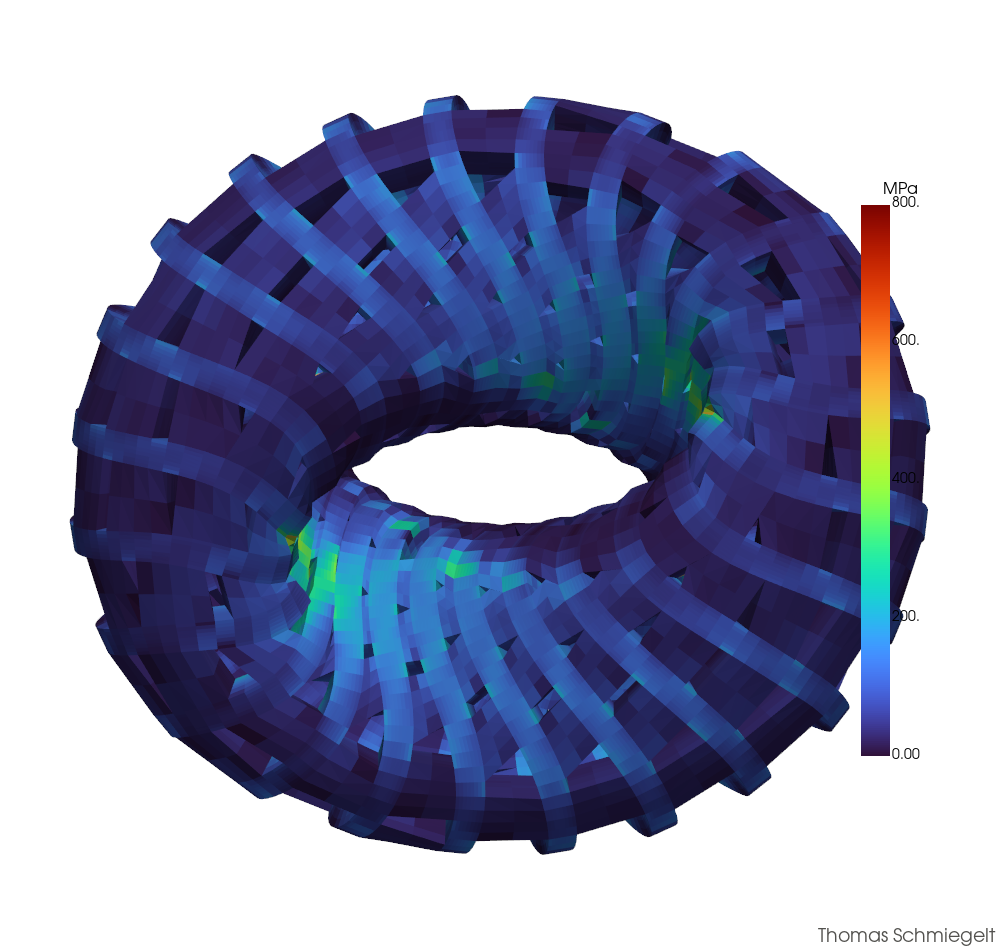
\includegraphics[width=\linewidth]{bilder/spannung_0008.png}\\\footnotesize Vergleichsspannung im Stahl (Draufsicht, 0–800 MPa)\end{minipage}\hfill
\begin{minipage}[t]{0.49\linewidth}\centering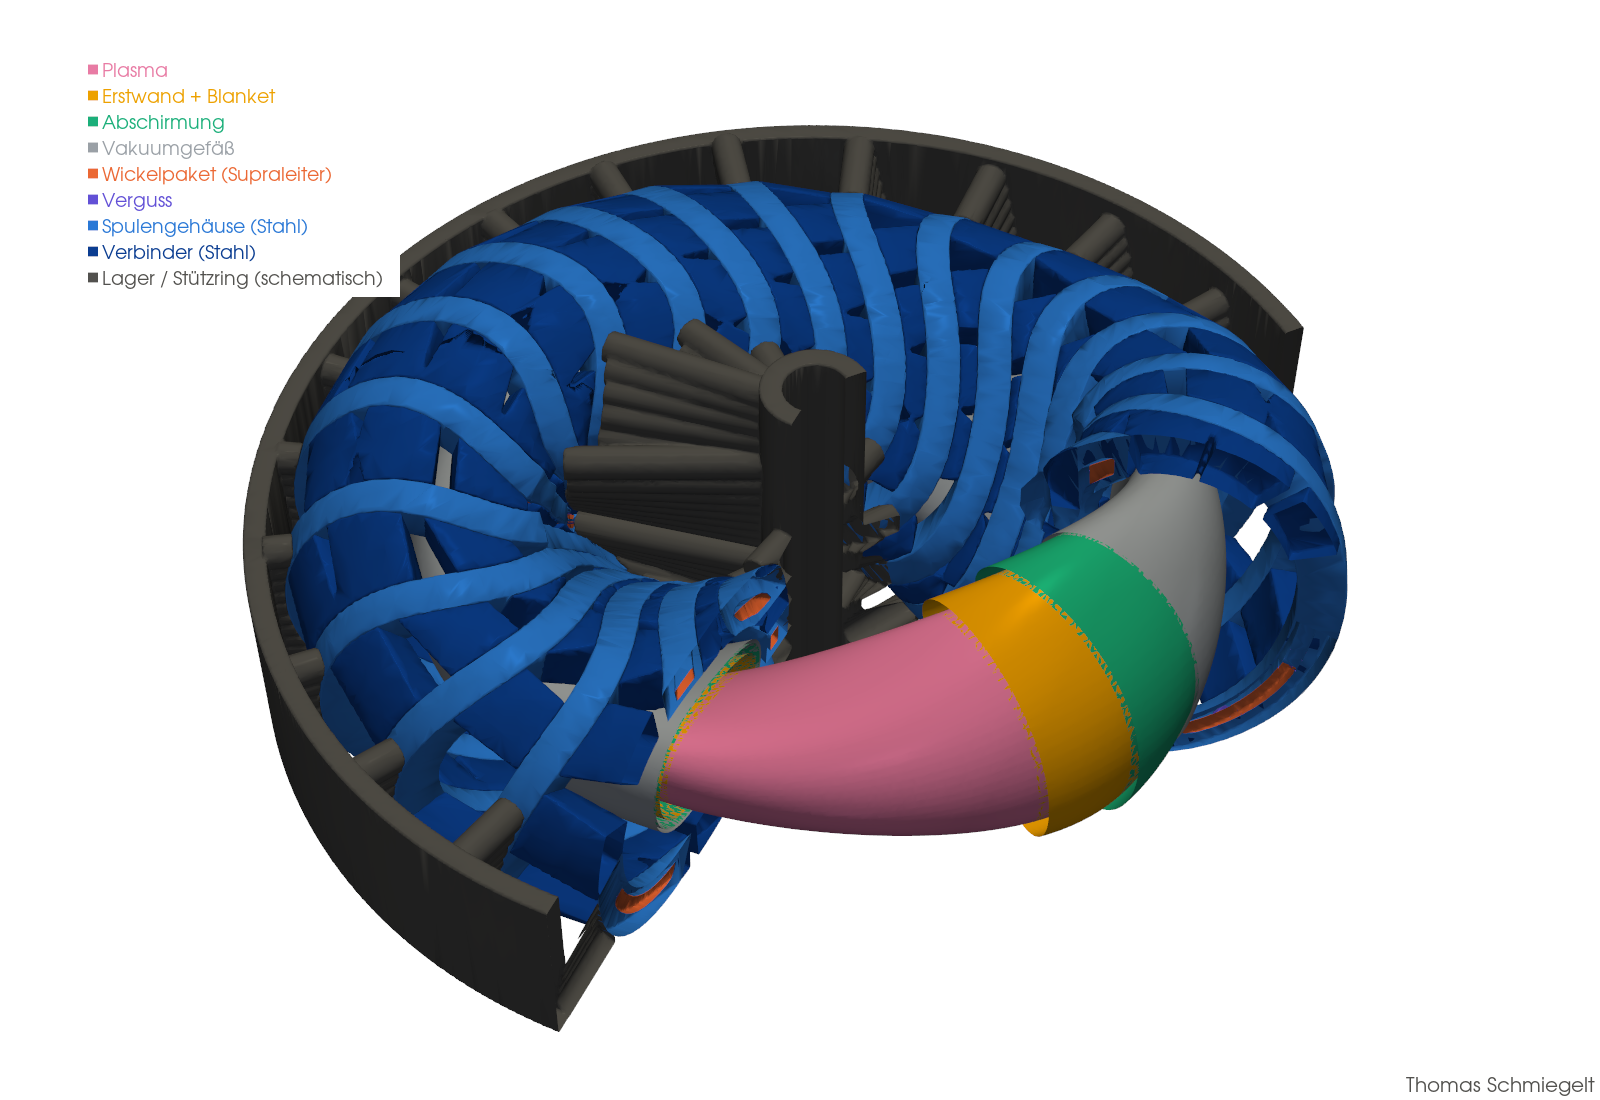
\includegraphics[width=\linewidth]{bilder/modell3d_0008_schnitt.png}\\\footnotesize PicoGK-Modell, Treppenschnitt\end{minipage}\hfill
\caption{Entwurf 0008}\end{figure}
\clearpage
\subsection{Entwurf 0014}\label{sb:0014}
\noindent\textbf{Urteil: }Zulässig (bereinigt), Rang 5 von 7; kleinste Reserve 25 \% (Stahl σ99).\par\smallskip
\begin{minipage}[t]{0.46\linewidth}\small\begin{tabular}[t]{@{}lr@{}}\toprule\multicolumn{2}{@{}l}{\textbf{Stellgrößen}}\\\midrule
Abstand Spule–Plasma & \num{0.233} \\
Spulen gesamt & 20 \\
Spulen je halbe Periode & \num{5} \\
Länge je Spule & \num{4.34} \\
Kraftziel & \num{0.025} \\
Wand innen & \num{0.35} \\
Seitenwand & \num{0.32} \\
Außenwand min. & \num{0.63} \\
Außenwand Zusatz & \num{0.29} \\
Verbindersteifigkeit & \num{196} \\
Verbinder je Paar & \num{11} \\
Lagerradius & \num{2.04} \\
\bottomrule\end{tabular}\end{minipage}\hfill
\begin{minipage}[t]{0.5\linewidth}\small\begin{tabular}[t]{@{}lr@{}}\toprule\multicolumn{2}{@{}l}{\textbf{Ergebnisse}}\\\midrule
$\sigma_{99}$ Stahl & \num{377} MPa \\
größtes Element & \num{1419} MPa \\
$P_m$ max. / 99 \% & \num{1369} / \num{459} MPa \\
$P_m+P_b$ max. & \num{1491} MPa \\
Verbinder σ99 & \num{243} MPa \\
Verformung max. & \num{18} mm \\
Dehnung Wickelpaket & \num{0.21} \% \\
Strom je Spule & \num{17.7} MA \\
Feld am Leiter & \num{16.9} T \\
Auslastung / Marge & \num{32} \% / \num{23} K \\
Feldfehler $B\cdot n$ & \num{2.21} ‰ \\
Freiraum Plasma–Gehäuse & \num{1.65} m \\
Kernheizung / Fluenz & \num{8} W/m³ / 6.5e16 \\
Stahl Gehäuse + Verbinder & \num{12.5} + \num{15.5} kt \\
Verbinder gebaut & 212 \\
\bottomrule\end{tabular}\end{minipage}\par\medskip
\noindent\textit{Netzstudie ($\sigma_{99}$/max. in MPa): }doe1: 377/1419; 1,5× Stationen: 549/3814; Wand 3 Zellen: 375/1639.\par\smallskip
\begin{figure}[H]\centering
\begin{minipage}[t]{0.49\linewidth}\centering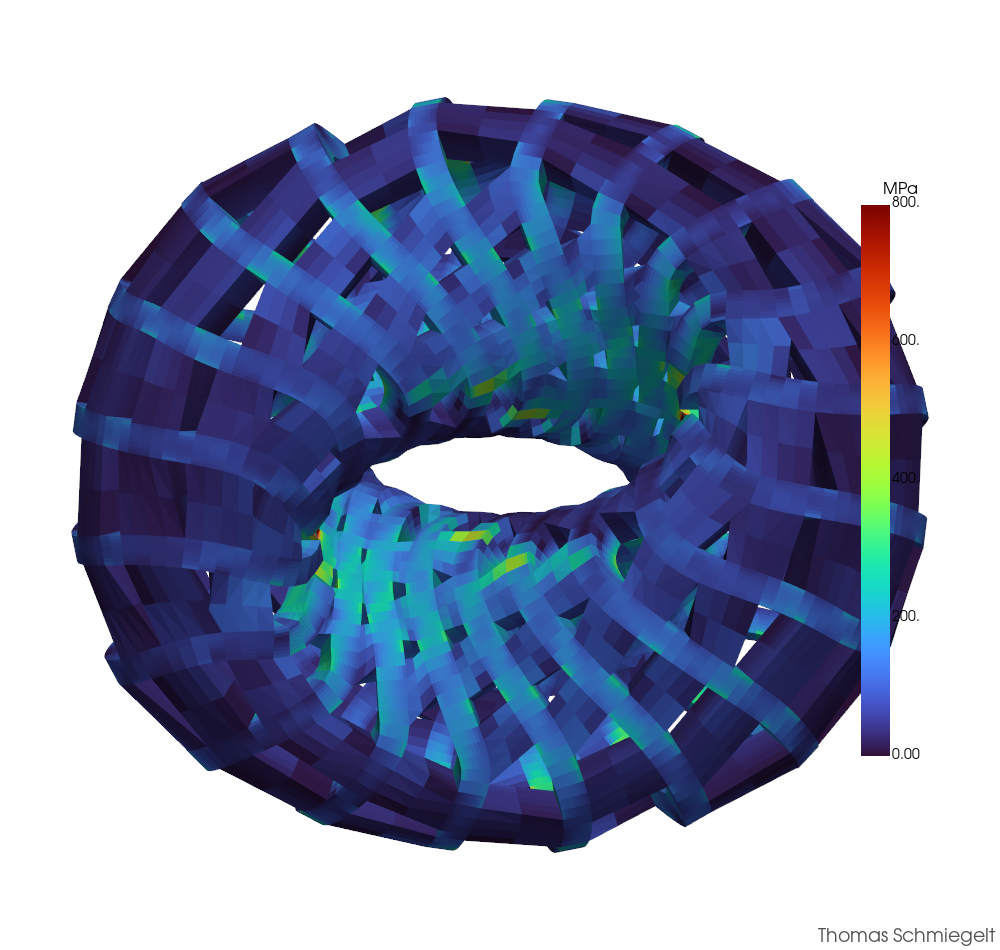
\includegraphics[width=\linewidth]{bilder/spannung_0014.png}\\\footnotesize Vergleichsspannung im Stahl (Draufsicht, 0–800 MPa)\end{minipage}\hfill
\begin{minipage}[t]{0.49\linewidth}\centering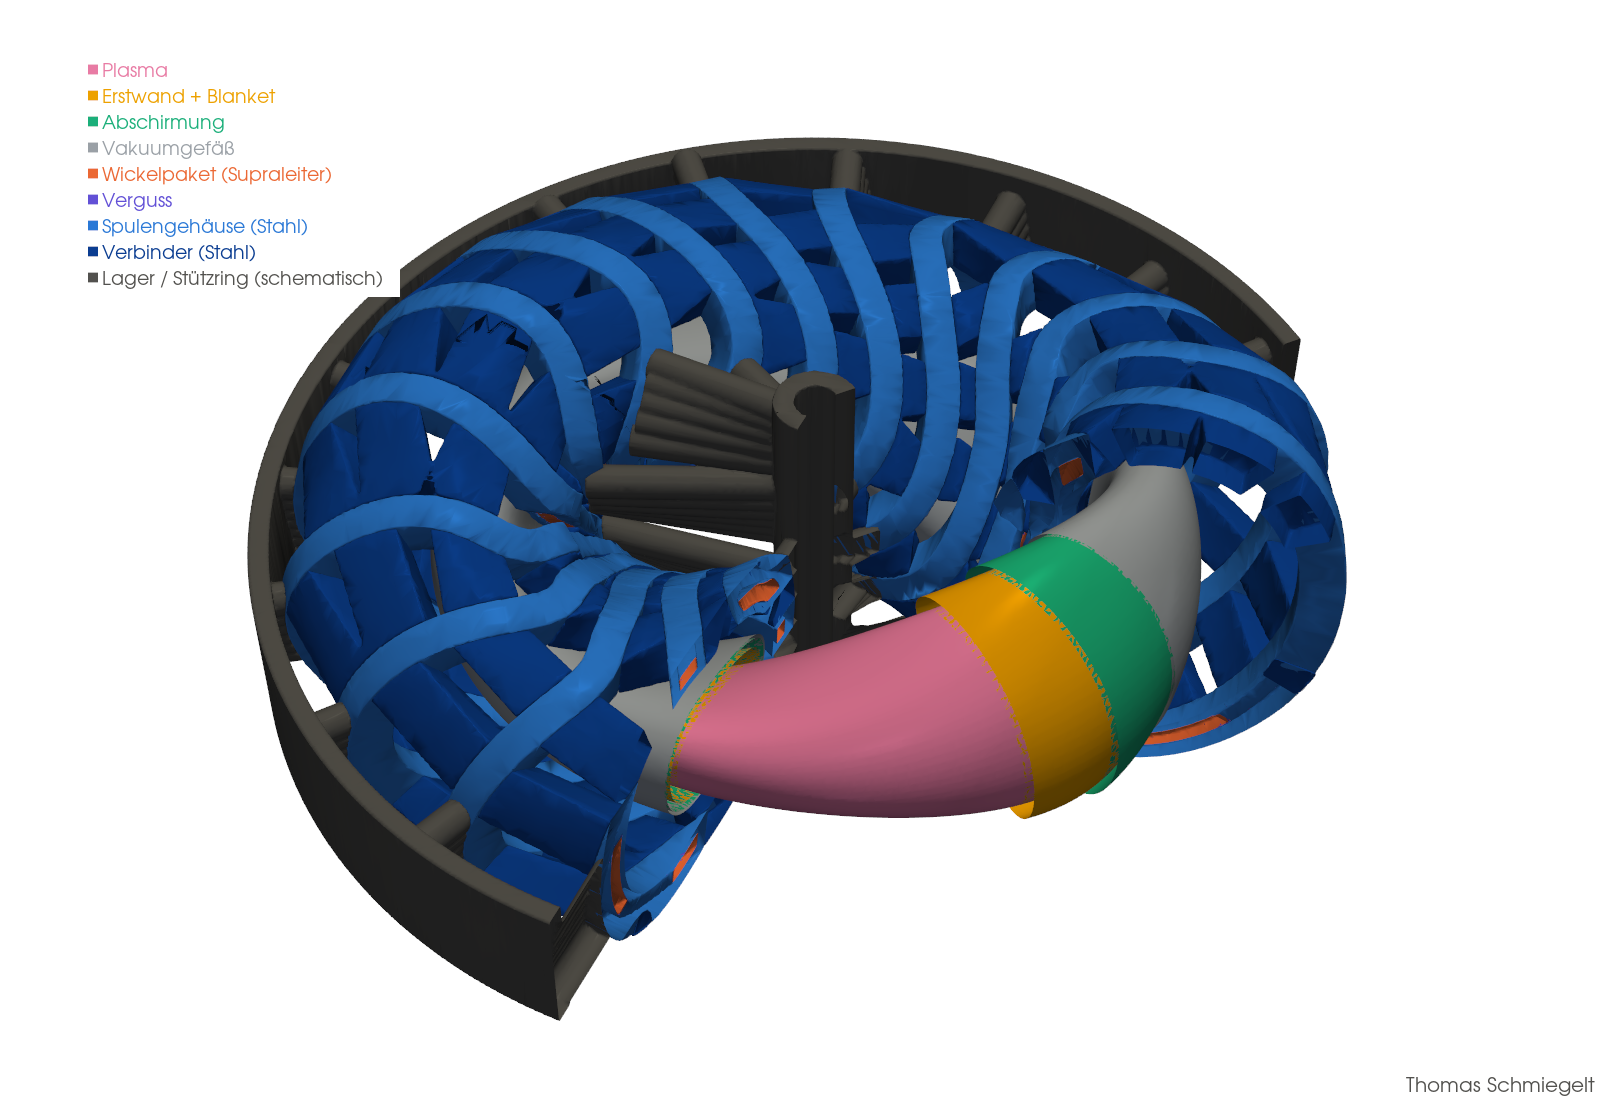
\includegraphics[width=\linewidth]{bilder/modell3d_0014_schnitt.png}\\\footnotesize PicoGK-Modell, Treppenschnitt\end{minipage}\hfill
\caption{Entwurf 0014}\end{figure}
\clearpage
\subsection{Entwurf 0017}\label{sb:0017}
\noindent\textbf{Urteil: }Zulässig (bereinigt), Rang 6 von 7; kleinste Reserve 20 \% (Platz Package).\par\smallskip
\begin{minipage}[t]{0.46\linewidth}\small\begin{tabular}[t]{@{}lr@{}}\toprule\multicolumn{2}{@{}l}{\textbf{Stellgrößen}}\\\midrule
Abstand Spule–Plasma & \num{0.220} \\
Spulen gesamt & 24 \\
Spulen je halbe Periode & \num{6} \\
Länge je Spule & \num{3.77} \\
Kraftziel & \num{0.019} \\
Wand innen & \num{0.60} \\
Seitenwand & \num{0.37} \\
Außenwand min. & \num{0.43} \\
Außenwand Zusatz & \num{0.32} \\
Verbindersteifigkeit & \num{29} \\
Verbinder je Paar & \num{7} \\
Lagerradius & \num{3.47} \\
\bottomrule\end{tabular}\end{minipage}\hfill
\begin{minipage}[t]{0.5\linewidth}\small\begin{tabular}[t]{@{}lr@{}}\toprule\multicolumn{2}{@{}l}{\textbf{Ergebnisse}}\\\midrule
$\sigma_{99}$ Stahl & \num{389} MPa \\
größtes Element & \num{1721} MPa \\
$P_m$ max. / 99 \% & \num{1631} / \num{448} MPa \\
$P_m+P_b$ max. & \num{1813} MPa \\
Verbinder σ99 & \num{131} MPa \\
Verformung max. & \num{31} mm \\
Dehnung Wickelpaket & \num{0.20} \% \\
Strom je Spule & \num{14.7} MA \\
Feld am Leiter & \num{16.0} T \\
Auslastung / Marge & \num{30} \% / \num{24} K \\
Feldfehler $B\cdot n$ & \num{1.66} ‰ \\
Freiraum Plasma–Gehäuse & \num{1.30} m \\
Kernheizung / Fluenz & \num{245} W/m³ / 2.0e18 \\
Stahl Gehäuse + Verbinder & \num{13.9} + \num{8.7} kt \\
Verbinder gebaut & 162 \\
\bottomrule\end{tabular}\end{minipage}\par\medskip
\begin{figure}[H]\centering
\begin{minipage}[t]{0.49\linewidth}\centering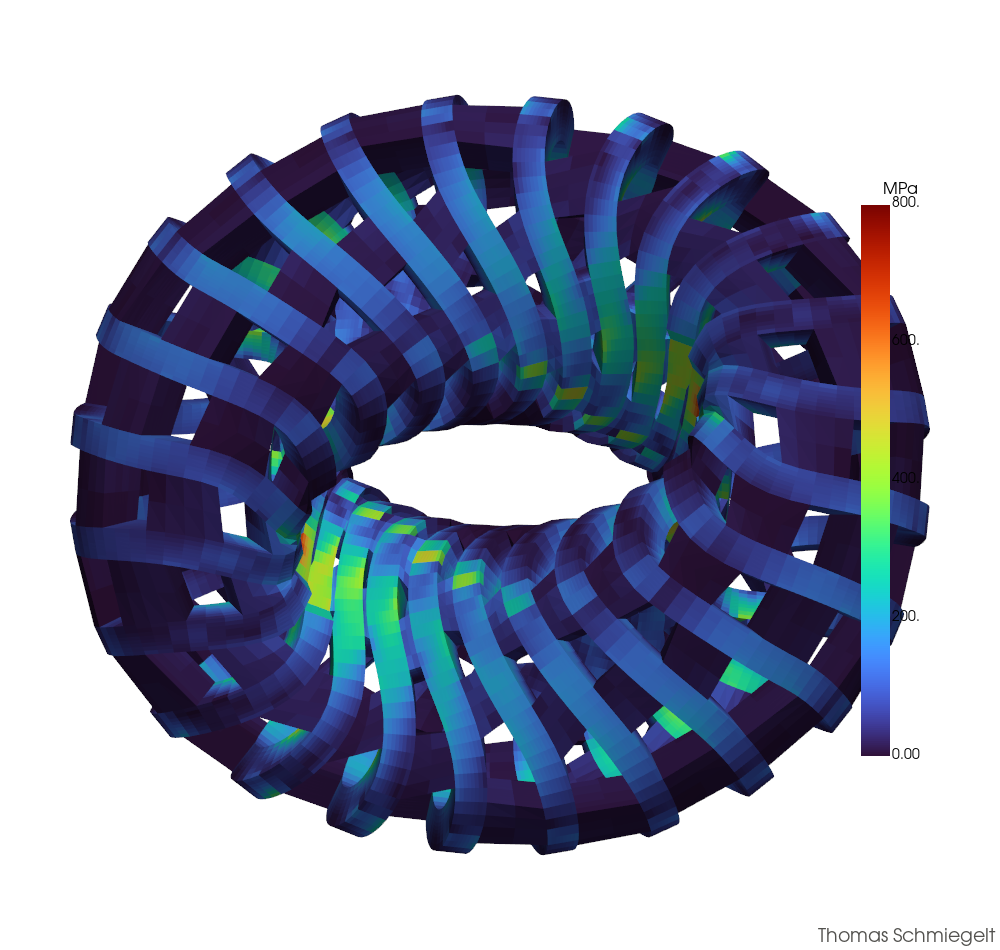
\includegraphics[width=\linewidth]{bilder/spannung_0017.png}\\\footnotesize Vergleichsspannung im Stahl (Draufsicht, 0–800 MPa)\end{minipage}\hfill
\begin{minipage}[t]{0.49\linewidth}\centering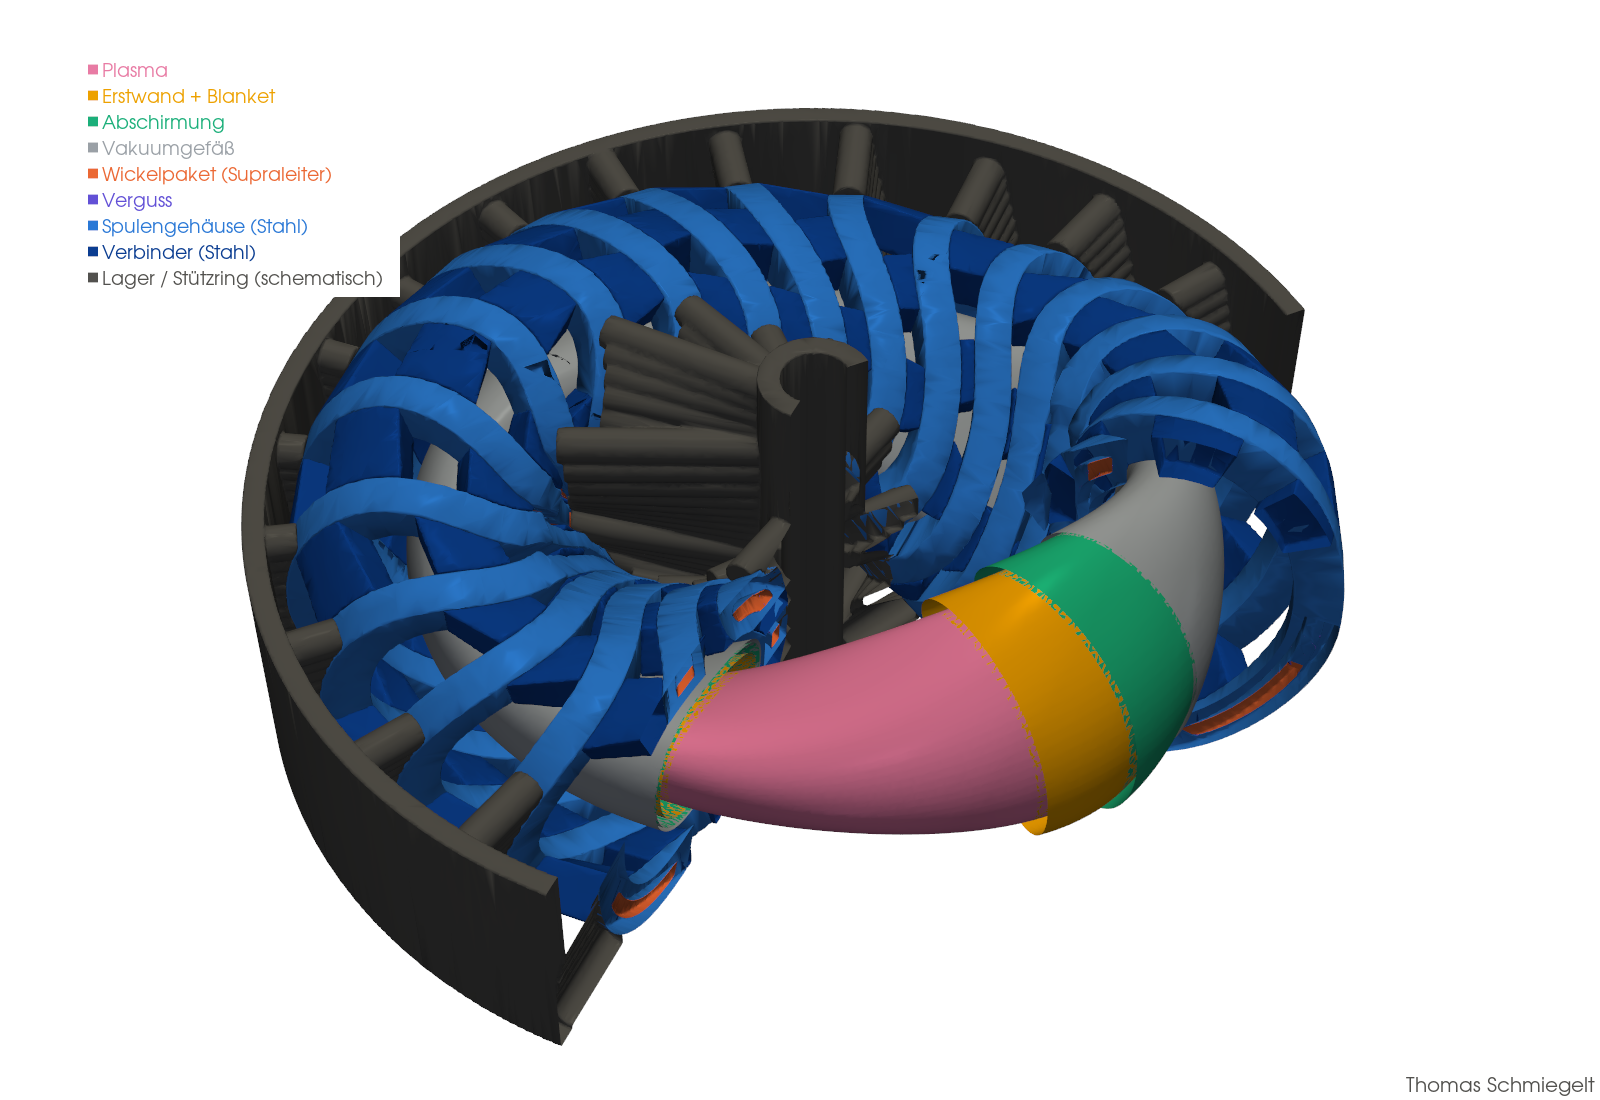
\includegraphics[width=\linewidth]{bilder/modell3d_0017_schnitt.png}\\\footnotesize PicoGK-Modell, Treppenschnitt\end{minipage}\hfill
\caption{Entwurf 0017}\end{figure}
\clearpage
\subsection{Entwurf 0157}\label{sb:0157}
\noindent\textbf{Urteil: }Zulässig (bereinigt), Rang 7 von 7; kleinste Reserve 2 \% (Stahl σ99).\par\smallskip
\begin{minipage}[t]{0.46\linewidth}\small\begin{tabular}[t]{@{}lr@{}}\toprule\multicolumn{2}{@{}l}{\textbf{Stellgrößen}}\\\midrule
Abstand Spule–Plasma & \num{0.218} \\
Spulen gesamt & 20 \\
Spulen je halbe Periode & \num{5} \\
Länge je Spule & \num{4.09} \\
Kraftziel & \num{0.020} \\
Wand innen & \num{0.49} \\
Seitenwand & \num{0.25} \\
Außenwand min. & \num{0.58} \\
Außenwand Zusatz & \num{0.02} \\
Verbindersteifigkeit & \num{158} \\
Verbinder je Paar & \num{6} \\
Lagerradius & \num{3.06} \\
\bottomrule\end{tabular}\end{minipage}\hfill
\begin{minipage}[t]{0.5\linewidth}\small\begin{tabular}[t]{@{}lr@{}}\toprule\multicolumn{2}{@{}l}{\textbf{Ergebnisse}}\\\midrule
$\sigma_{99}$ Stahl & \num{492} MPa \\
größtes Element & \num{1658} MPa \\
$P_m$ max. / 99 \% & \num{1405} / \num{519} MPa \\
$P_m+P_b$ max. & \num{1920} MPa \\
Verbinder σ99 & \num{335} MPa \\
Verformung max. & \num{34} mm \\
Dehnung Wickelpaket & \num{0.22} \% \\
Strom je Spule & \num{17.7} MA \\
Feld am Leiter & \num{16.5} T \\
Auslastung / Marge & \num{31} \% / \num{23} K \\
Feldfehler $B\cdot n$ & \num{2.37} ‰ \\
Freiraum Plasma–Gehäuse & \num{1.35} m \\
Kernheizung / Fluenz & \num{142} W/m³ / 1.2e18 \\
Stahl Gehäuse + Verbinder & \num{10.1} + \num{7.5} kt \\
Verbinder gebaut & 118 \\
\bottomrule\end{tabular}\end{minipage}\par\medskip
\begin{figure}[H]\centering
\begin{minipage}[t]{0.49\linewidth}\centering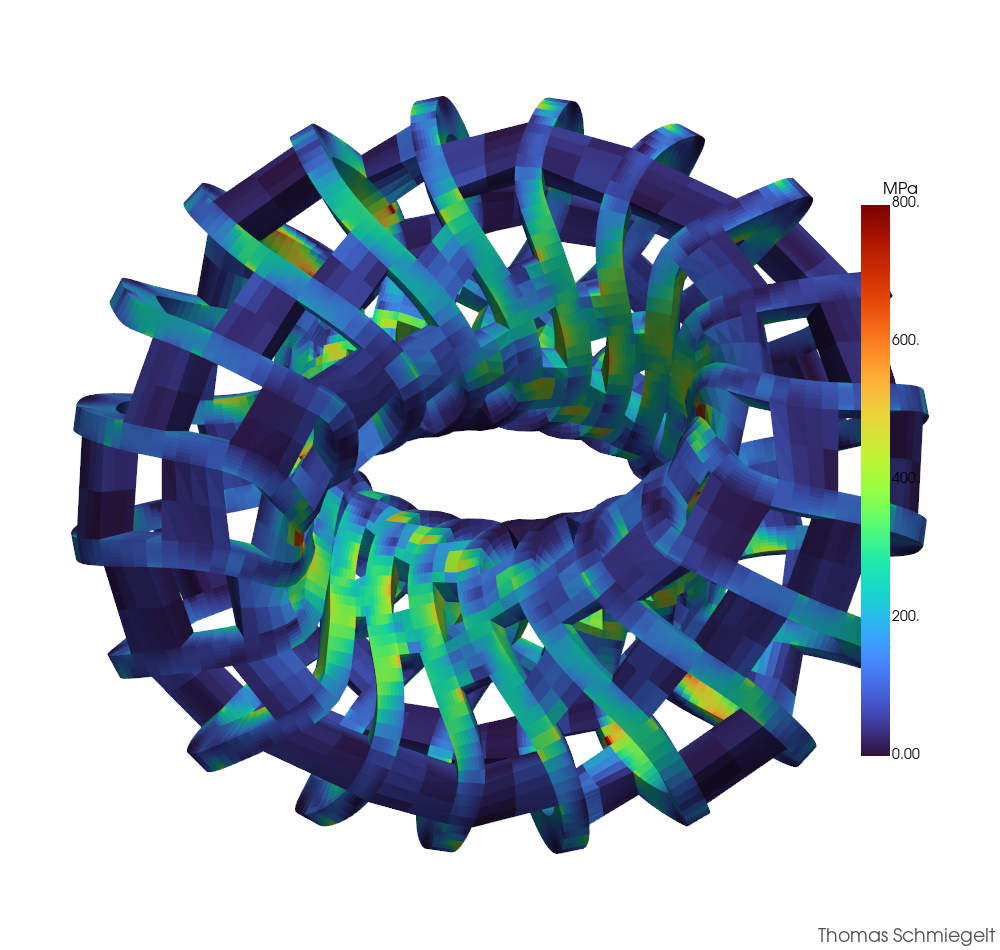
\includegraphics[width=\linewidth]{bilder/spannung_0157.png}\\\footnotesize Vergleichsspannung im Stahl (Draufsicht, 0–800 MPa)\end{minipage}\hfill
\begin{minipage}[t]{0.49\linewidth}\centering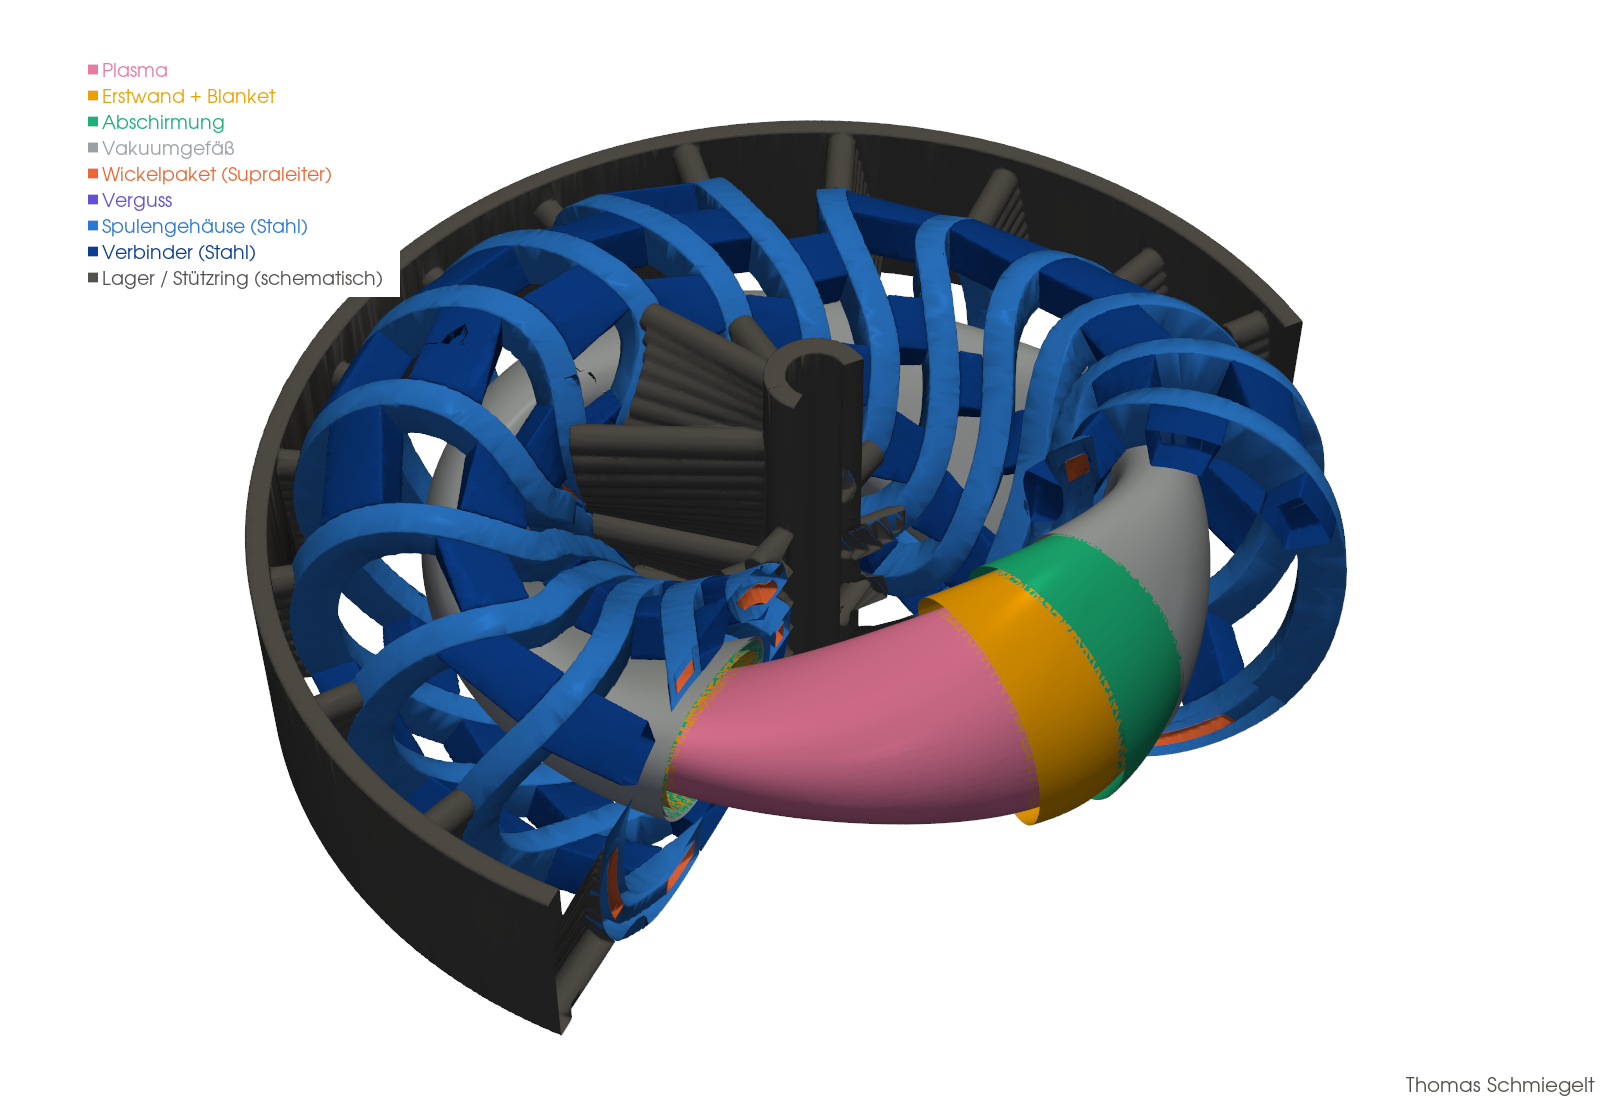
\includegraphics[width=\linewidth]{bilder/modell3d_0157_schnitt.png}\\\footnotesize PicoGK-Modell, Treppenschnitt\end{minipage}\hfill
\caption{Entwurf 0157}\end{figure}
\clearpage
\subsection{Entwurf 0063}\label{sb:0063}
\noindent\textbf{Urteil: }In doe1 zulässig, mit Standardnetz nicht mehr: Engpass Dehnung Wickelpaket (Reserve -24 \%).\par\smallskip
\begin{minipage}[t]{0.46\linewidth}\small\begin{tabular}[t]{@{}lr@{}}\toprule\multicolumn{2}{@{}l}{\textbf{Stellgrößen}}\\\midrule
Abstand Spule–Plasma & \num{0.177} \\
Spulen gesamt & 20 \\
Spulen je halbe Periode & \num{5} \\
Länge je Spule & \num{4.45} \\
Kraftziel & \num{0.000} \\
Wand innen & \num{0.59} \\
Seitenwand & \num{0.35} \\
Außenwand min. & \num{0.69} \\
Außenwand Zusatz & \num{0.44} \\
Verbindersteifigkeit & \num{43} \\
Verbinder je Paar & \num{14} \\
Lagerradius & \num{1.71} \\
\bottomrule\end{tabular}\end{minipage}\hfill
\begin{minipage}[t]{0.5\linewidth}\small\begin{tabular}[t]{@{}lr@{}}\toprule\multicolumn{2}{@{}l}{\textbf{Ergebnisse}}\\\midrule
$\sigma_{99}$ Stahl & \num{595} MPa \\
größtes Element & \num{4265} MPa \\
$P_m$ max. / 99 \% & \num{4261} / \num{942} MPa \\
$P_m+P_b$ max. & \num{4270} MPa \\
Verbinder σ99 & \num{200} MPa \\
Verformung max. & \num{81} mm \\
Dehnung Wickelpaket & \num{0.37} \% \\
Strom je Spule & \num{17.7} MA \\
Feld am Leiter & \num{17.5} T \\
Auslastung / Marge & \num{33} \% / \num{22} K \\
Feldfehler $B\cdot n$ & \num{0.75} ‰ \\
Freiraum Plasma–Gehäuse & \num{1.53} m \\
Kernheizung / Fluenz & \num{24} W/m³ / 2.0e17 \\
Stahl Gehäuse + Verbinder & \num{16.7} + \num{24.2} kt \\
Verbinder gebaut & 252 \\
\bottomrule\end{tabular}\end{minipage}\par\medskip
\noindent\textit{Netzstudie ($\sigma_{99}$/max. in MPa): }doe1: 369/2016; Standard: 595/4265.\par\smallskip
\begin{figure}[H]\centering
\begin{minipage}[t]{0.49\linewidth}\centering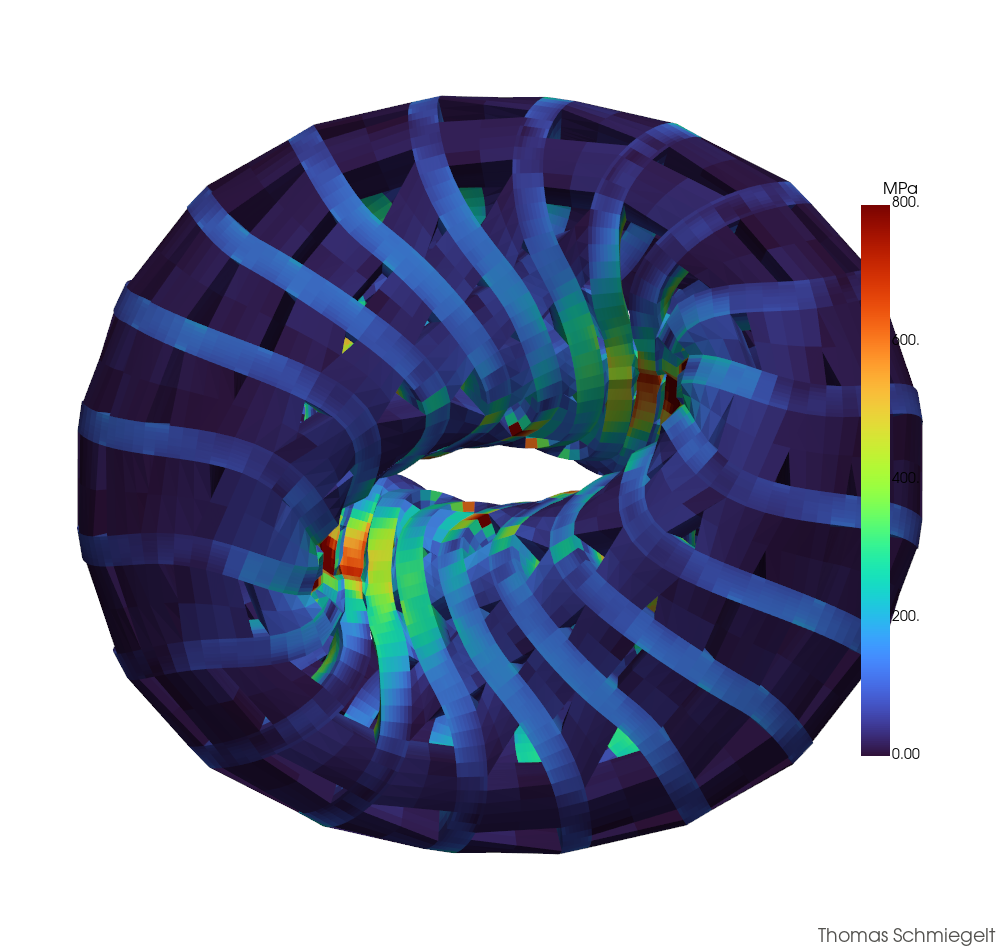
\includegraphics[width=\linewidth]{bilder/spannung_0063.png}\\\footnotesize Vergleichsspannung im Stahl (Draufsicht, 0–800 MPa)\end{minipage}\hfill
\begin{minipage}[t]{0.49\linewidth}\centering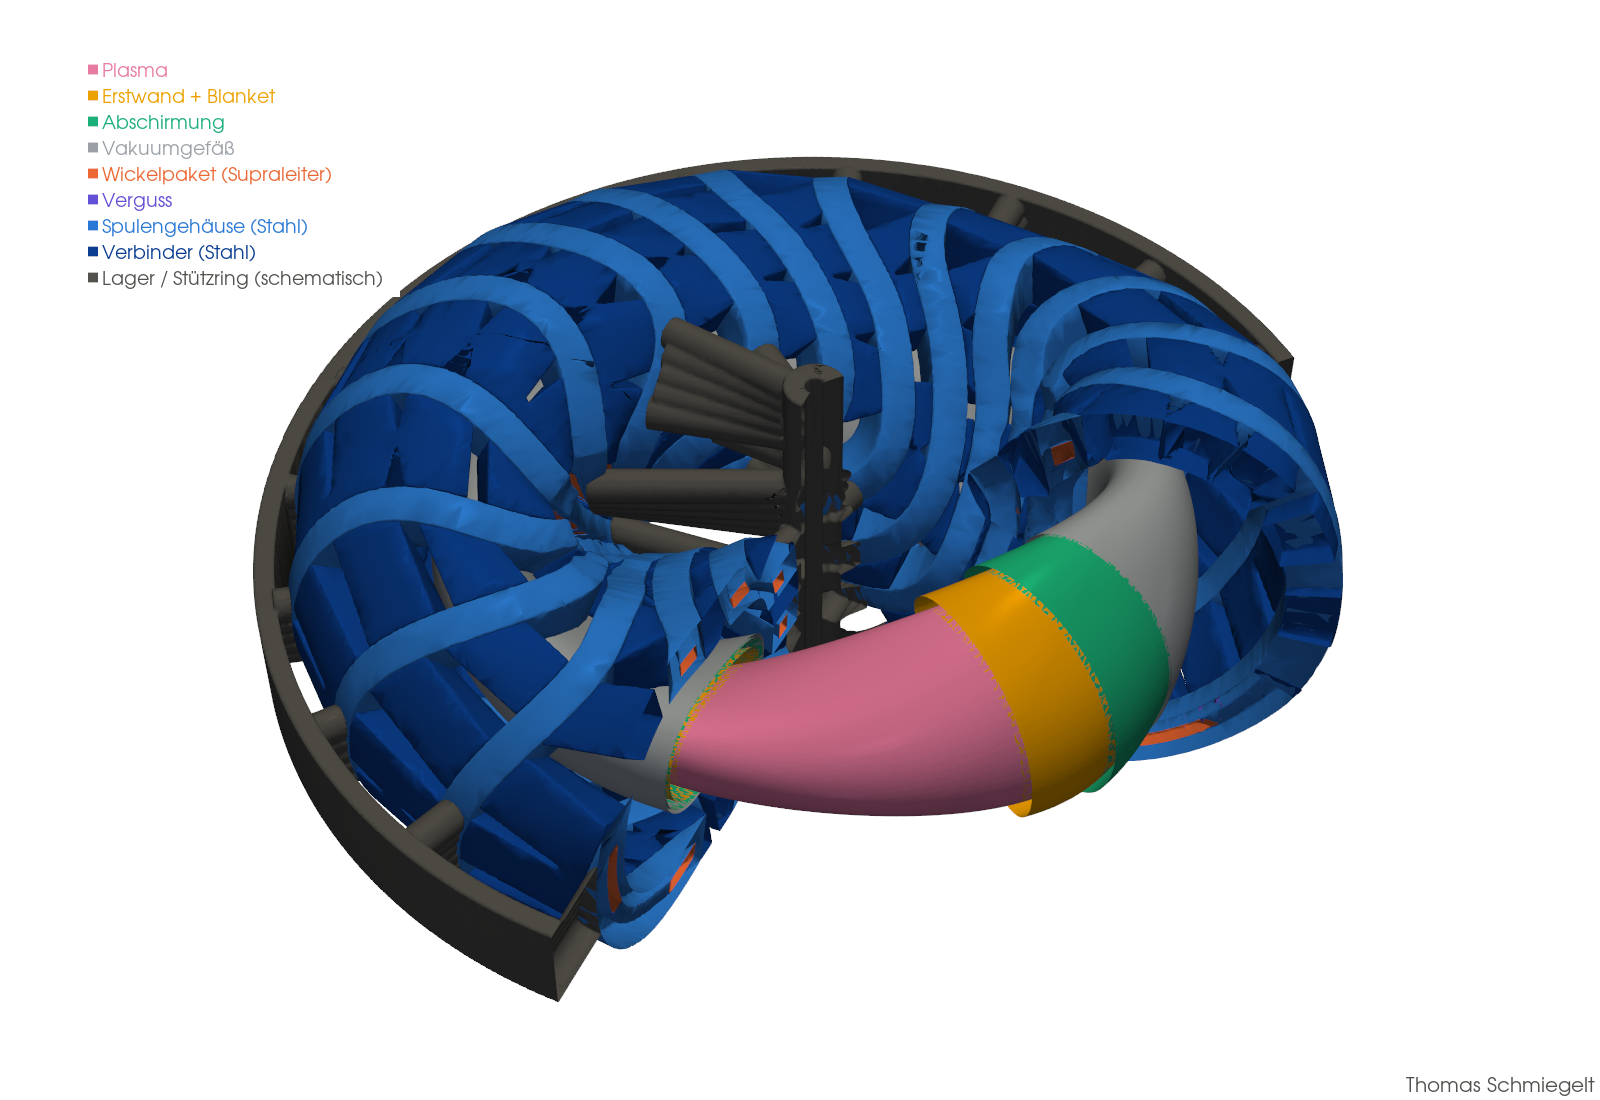
\includegraphics[width=\linewidth]{bilder/modell3d_0063_schnitt.png}\\\footnotesize PicoGK-Modell, Treppenschnitt\end{minipage}\hfill
\caption{Entwurf 0063}\end{figure}
\clearpage
\subsection{Entwurf 0136}\label{sb:0136}
\noindent\textbf{Urteil: }In doe1 zulässig, mit Standardnetz nicht mehr: Engpass Stahl σ99 (Reserve -15 \%).\par\smallskip
\begin{minipage}[t]{0.46\linewidth}\small\begin{tabular}[t]{@{}lr@{}}\toprule\multicolumn{2}{@{}l}{\textbf{Stellgrößen}}\\\midrule
Abstand Spule–Plasma & \num{0.232} \\
Spulen gesamt & 20 \\
Spulen je halbe Periode & \num{5} \\
Länge je Spule & \num{4.51} \\
Kraftziel & \num{0.012} \\
Wand innen & \num{0.16} \\
Seitenwand & \num{0.30} \\
Außenwand min. & \num{0.57} \\
Außenwand Zusatz & \num{0.22} \\
Verbindersteifigkeit & \num{21} \\
Verbinder je Paar & \num{13} \\
Lagerradius & \num{3.12} \\
\bottomrule\end{tabular}\end{minipage}\hfill
\begin{minipage}[t]{0.5\linewidth}\small\begin{tabular}[t]{@{}lr@{}}\toprule\multicolumn{2}{@{}l}{\textbf{Ergebnisse}}\\\midrule
$\sigma_{99}$ Stahl & \num{577} MPa \\
größtes Element & \num{2238} MPa \\
$P_m$ max. / 99 \% & \num{2201} / \num{690} MPa \\
$P_m+P_b$ max. & \num{2291} MPa \\
Verbinder σ99 & \num{141} MPa \\
Verformung max. & \num{54} mm \\
Dehnung Wickelpaket & \num{0.30} \% \\
Strom je Spule & \num{17.7} MA \\
Feld am Leiter & \num{16.9} T \\
Auslastung / Marge & \num{32} \% / \num{23} K \\
Feldfehler $B\cdot n$ & \num{1.62} ‰ \\
Freiraum Plasma–Gehäuse & \num{1.84} m \\
Kernheizung / Fluenz & \num{1} W/m³ / 9.6e15 \\
Stahl Gehäuse + Verbinder & \num{10.0} + \num{16.3} kt \\
Verbinder gebaut & 254 \\
\bottomrule\end{tabular}\end{minipage}\par\medskip
\noindent\textit{Netzstudie ($\sigma_{99}$/max. in MPa): }doe1: 479/995; Standard: 577/2238.\par\smallskip
\begin{figure}[H]\centering
\begin{minipage}[t]{0.49\linewidth}\centering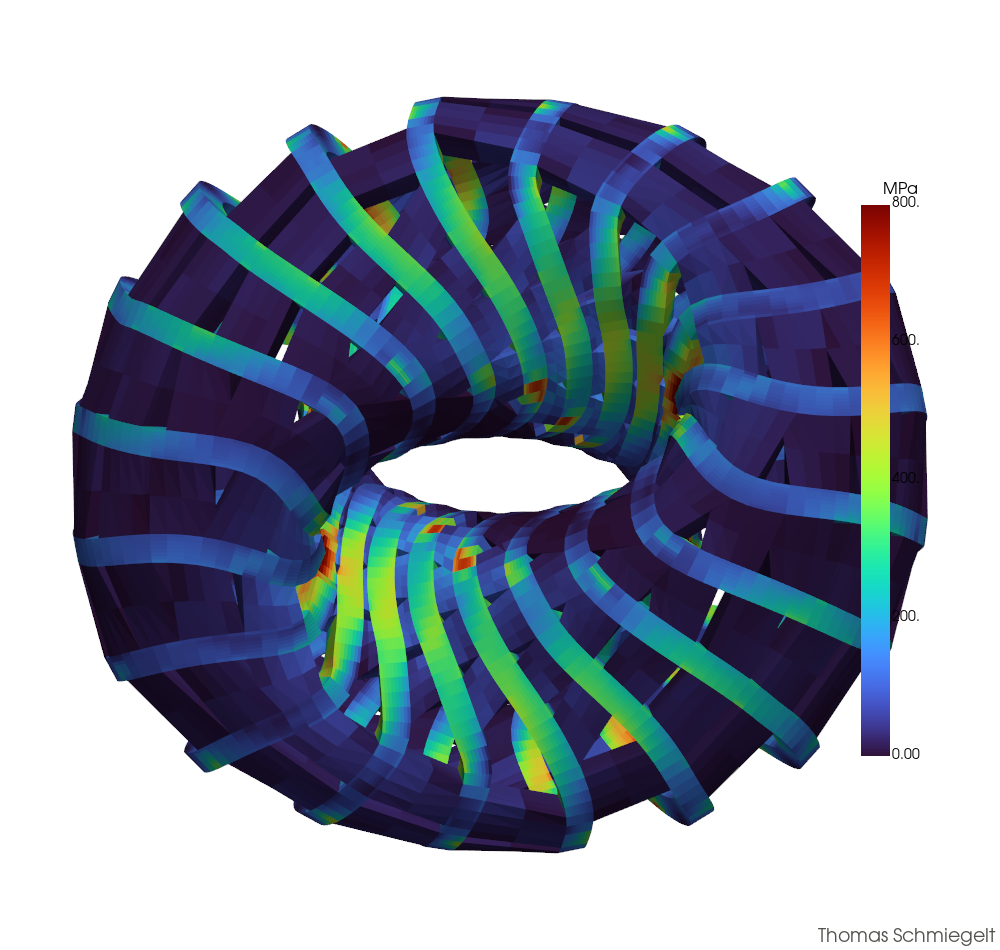
\includegraphics[width=\linewidth]{bilder/spannung_0136.png}\\\footnotesize Vergleichsspannung im Stahl (Draufsicht, 0–800 MPa)\end{minipage}\hfill
\begin{minipage}[t]{0.49\linewidth}\centering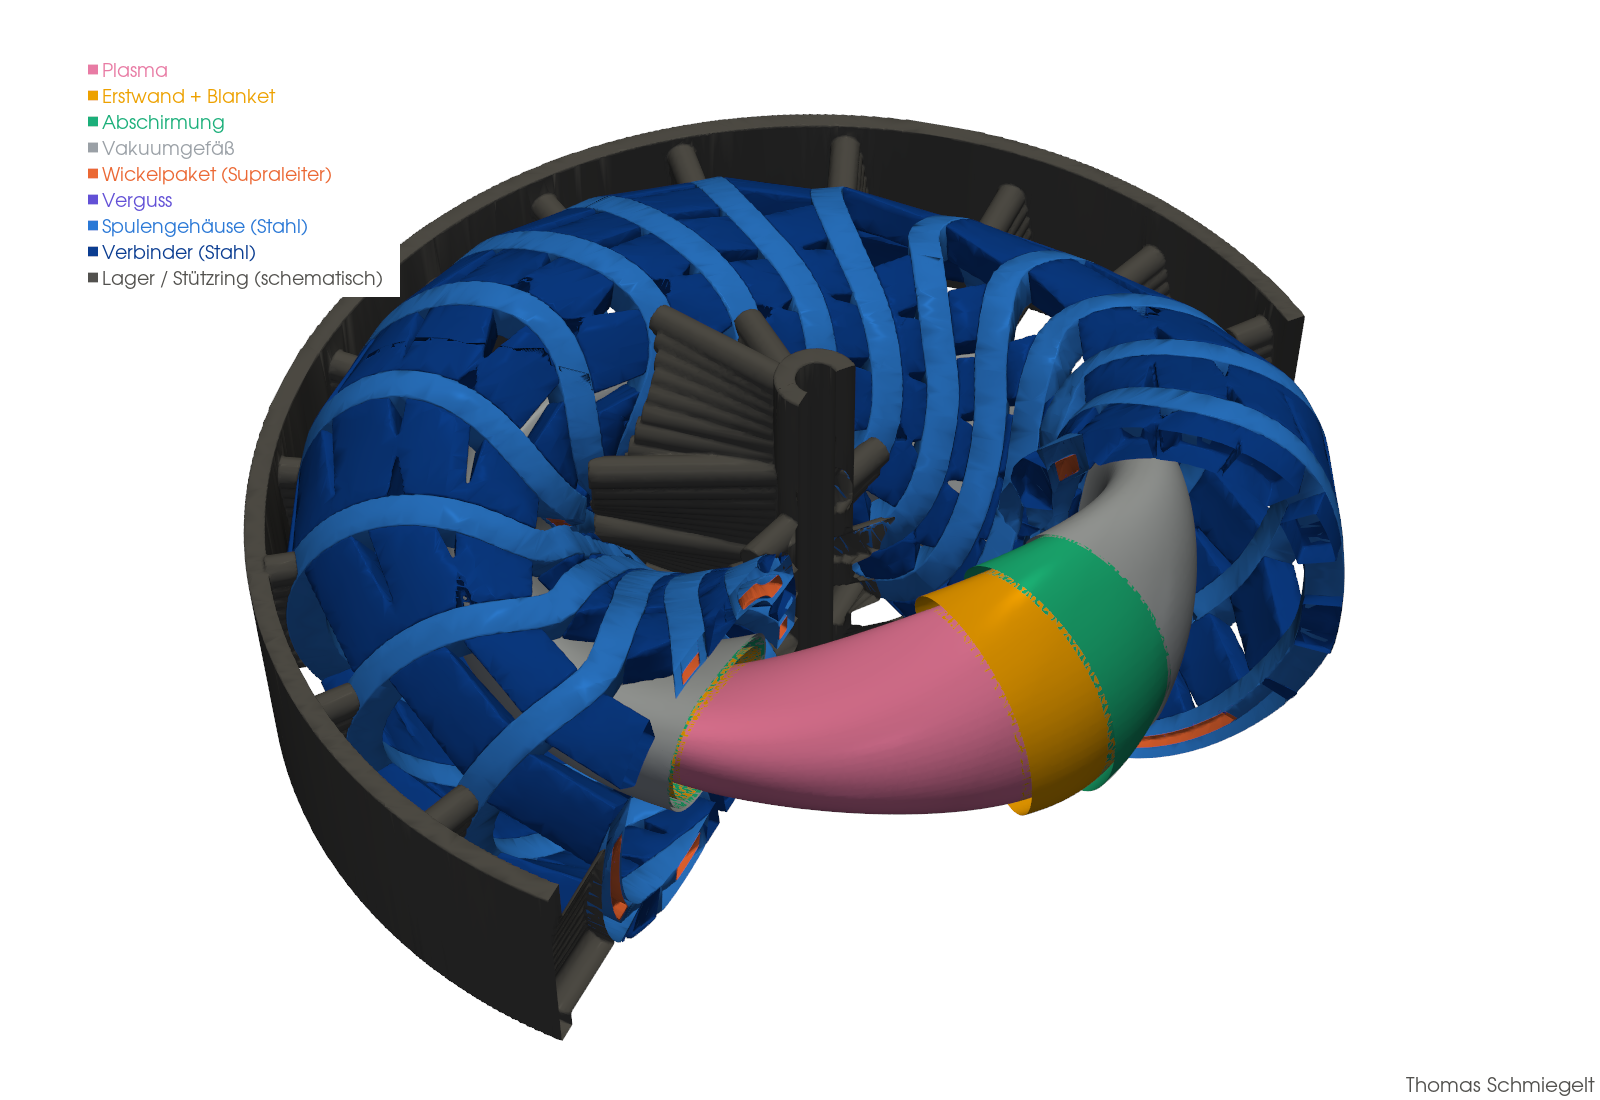
\includegraphics[width=\linewidth]{bilder/modell3d_0136_schnitt.png}\\\footnotesize PicoGK-Modell, Treppenschnitt\end{minipage}\hfill
\caption{Entwurf 0136}\end{figure}
\clearpage
\subsection{Vorschlag V3 des Ersatzmodells}\label{sb:V3}
\noindent\textbf{Urteil: }Vorschlag des Ersatzmodells (Abschnitt~\ref{sec:ersatz1}), zulässig; kleinste Reserve 35 \% (Feldfehler B·n).\par\smallskip
\begin{minipage}[t]{0.46\linewidth}\small\begin{tabular}[t]{@{}lr@{}}\toprule\multicolumn{2}{@{}l}{\textbf{Stellgrößen}}\\\midrule
Abstand Spule–Plasma & \num{0.205} \\
Spulen gesamt & 24 \\
Spulen je halbe Periode & \num{6} \\
Länge je Spule & \num{4.15} \\
Kraftziel & \num{0.022} \\
Wand innen & \num{0.20} \\
Seitenwand & \num{0.24} \\
Außenwand min. & \num{0.77} \\
Außenwand Zusatz & \num{0.48} \\
Verbindersteifigkeit & \num{176} \\
Verbinder je Paar & \num{11} \\
Lagerradius & \num{3.02} \\
\bottomrule\end{tabular}\end{minipage}\hfill
\begin{minipage}[t]{0.5\linewidth}\small\begin{tabular}[t]{@{}lr@{}}\toprule\multicolumn{2}{@{}l}{\textbf{Ergebnisse}}\\\midrule
$\sigma_{99}$ Stahl & \num{272} MPa \\
größtes Element & \num{656} MPa \\
$P_m$ max. / 99 \% & \num{621} / \num{302} MPa \\
$P_m+P_b$ max. & \num{724} MPa \\
Verbinder σ99 & \num{178} MPa \\
Verformung max. & \num{13} mm \\
Dehnung Wickelpaket & \num{0.13} \% \\
Strom je Spule & \num{14.7} MA \\
Feld am Leiter & \num{15.6} T \\
Auslastung / Marge & \num{30} \% / \num{24} K \\
Feldfehler $B\cdot n$ & \num{1.96} ‰ \\
Freiraum Plasma–Gehäuse & \num{1.54} m \\
Kernheizung / Fluenz & \num{22} W/m³ / 1.8e17 \\
Stahl Gehäuse + Verbinder & \num{12.3} + \num{16.8} kt \\
Verbinder gebaut & 256 \\
\bottomrule\end{tabular}\end{minipage}\par\medskip
\noindent\textit{Netzstudie ($\sigma_{99}$/max. in MPa): }Standard: 272/656; 1,5× Stationen: 394/1841.\par\smallskip
\begin{figure}[H]\centering
\begin{minipage}[t]{0.49\linewidth}\centering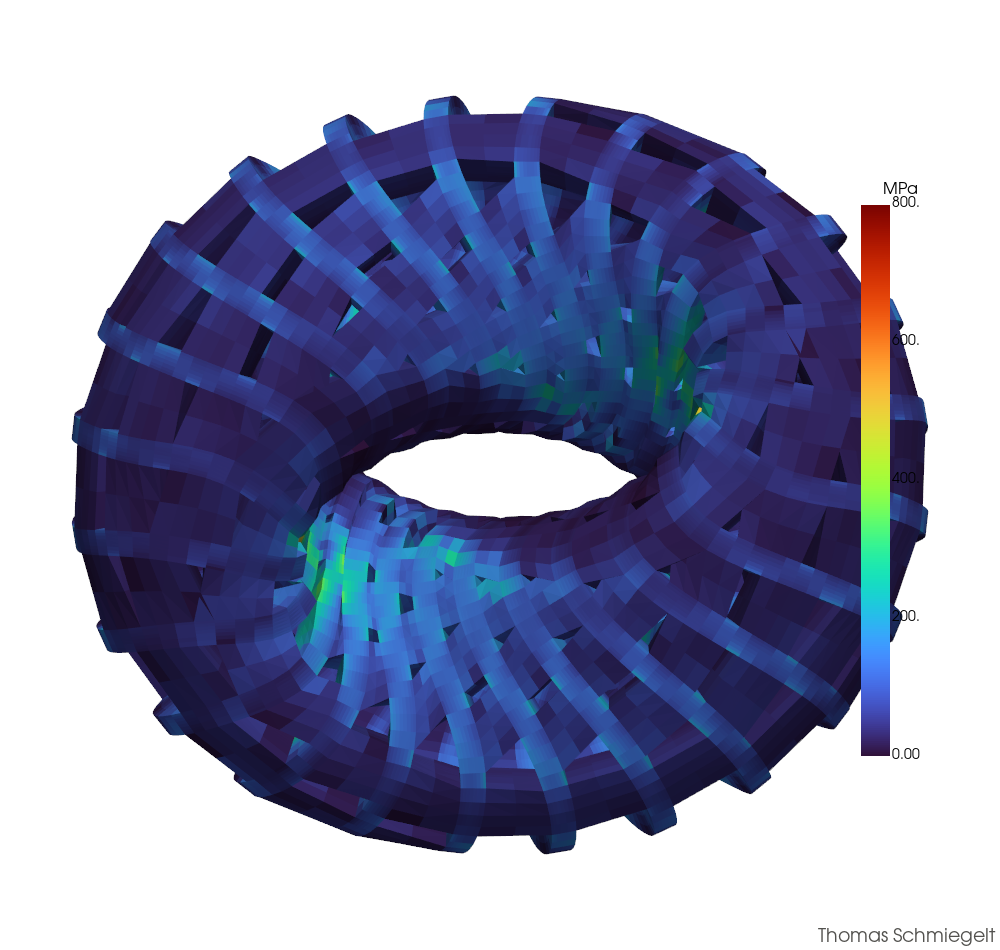
\includegraphics[width=\linewidth]{bilder/spannung_V3.png}\\\footnotesize Vergleichsspannung im Stahl (Draufsicht, 0–800 MPa)\end{minipage}\hfill
\begin{minipage}[t]{0.49\linewidth}\centering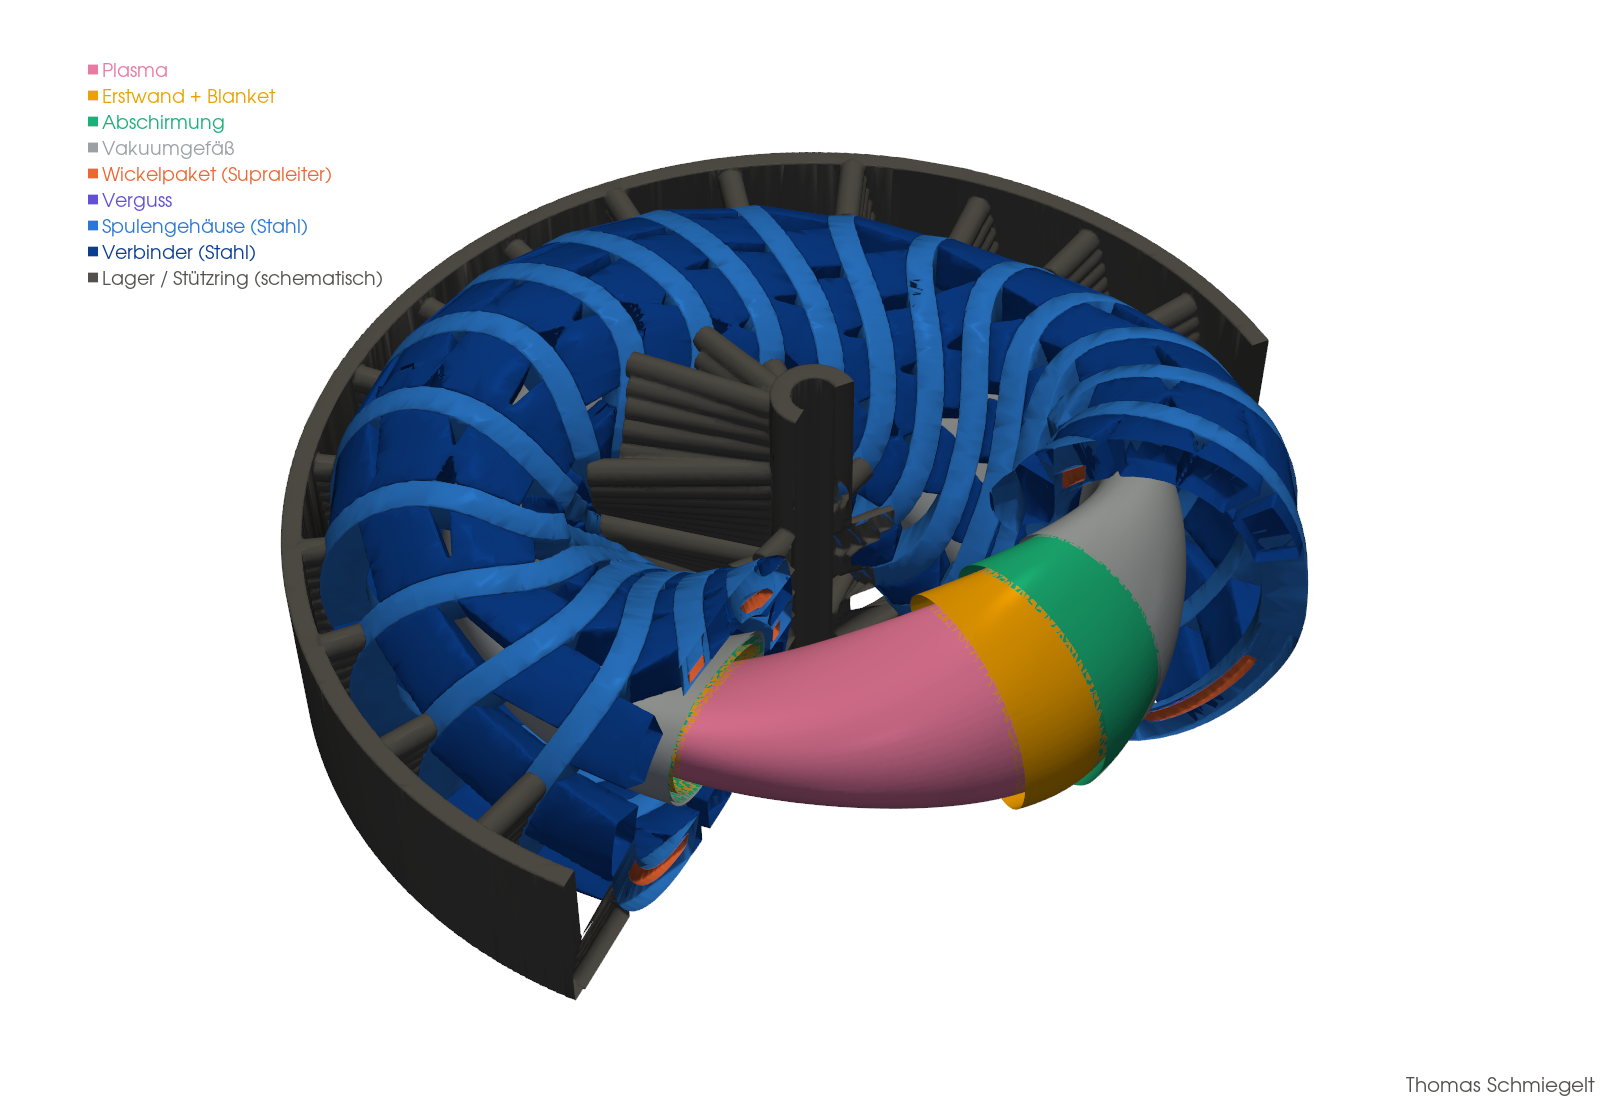
\includegraphics[width=\linewidth]{bilder/modell3d_V3_schnitt.png}\\\footnotesize PicoGK-Modell, Treppenschnitt\end{minipage}\hfill
\caption{Vorschlag V3 des Ersatzmodells}\end{figure}
\clearpage
\subsection{Vorschlag V1 des Ersatzmodells}\label{sb:V1}
\noindent\textbf{Urteil: }Vorschlag des Ersatzmodells (Abschnitt~\ref{sec:ersatz1}), zulässig; kleinste Reserve 31 \% (Platz Package).\par\smallskip
\begin{minipage}[t]{0.46\linewidth}\small\begin{tabular}[t]{@{}lr@{}}\toprule\multicolumn{2}{@{}l}{\textbf{Stellgrößen}}\\\midrule
Abstand Spule–Plasma & \num{0.208} \\
Spulen gesamt & 24 \\
Spulen je halbe Periode & \num{6} \\
Länge je Spule & \num{3.98} \\
Kraftziel & \num{0.023} \\
Wand innen & \num{0.36} \\
Seitenwand & \num{0.32} \\
Außenwand min. & \num{0.77} \\
Außenwand Zusatz & \num{0.33} \\
Verbindersteifigkeit & \num{77} \\
Verbinder je Paar & \num{13} \\
Lagerradius & \num{3.41} \\
\bottomrule\end{tabular}\end{minipage}\hfill
\begin{minipage}[t]{0.5\linewidth}\small\begin{tabular}[t]{@{}lr@{}}\toprule\multicolumn{2}{@{}l}{\textbf{Ergebnisse}}\\\midrule
$\sigma_{99}$ Stahl & \num{220} MPa \\
größtes Element & \num{637} MPa \\
$P_m$ max. / 99 \% & \num{532} / \num{248} MPa \\
$P_m+P_b$ max. & \num{746} MPa \\
Verbinder σ99 & \num{111} MPa \\
Verformung max. & \num{11} mm \\
Dehnung Wickelpaket & \num{0.12} \% \\
Strom je Spule & \num{14.7} MA \\
Feld am Leiter & \num{15.6} T \\
Auslastung / Marge & \num{30} \% / \num{24} K \\
Feldfehler $B\cdot n$ & \num{1.87} ‰ \\
Freiraum Plasma–Gehäuse & \num{1.41} m \\
Kernheizung / Fluenz & \num{85} W/m³ / 7.1e17 \\
Stahl Gehäuse + Verbinder & \num{14.6} + \num{18.5} kt \\
Verbinder gebaut & 308 \\
\bottomrule\end{tabular}\end{minipage}\par\medskip
\noindent\textit{Netzstudie ($\sigma_{99}$/max. in MPa): }Standard: 220/637; 1,5× Stationen: 366/2185.\par\smallskip
\begin{figure}[H]\centering
\begin{minipage}[t]{0.49\linewidth}\centering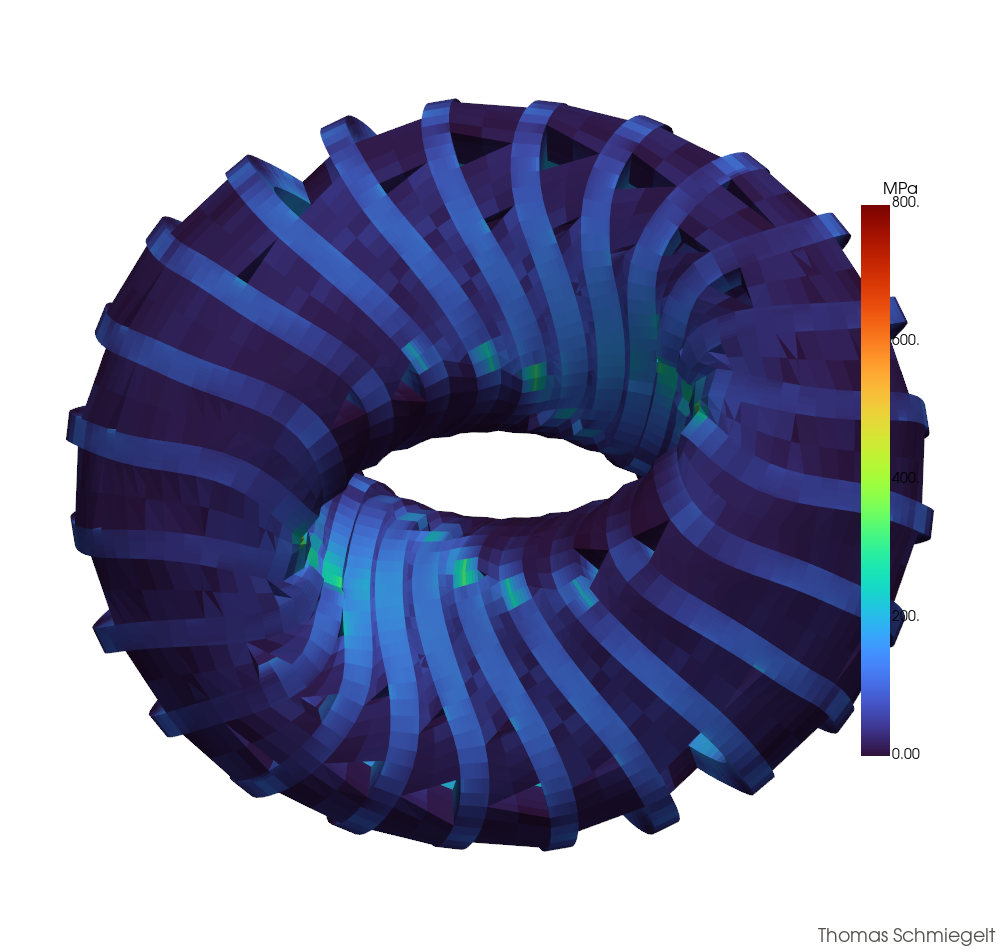
\includegraphics[width=\linewidth]{bilder/spannung_V1.png}\\\footnotesize Vergleichsspannung im Stahl (Draufsicht, 0–800 MPa)\end{minipage}\hfill
\begin{minipage}[t]{0.49\linewidth}\centering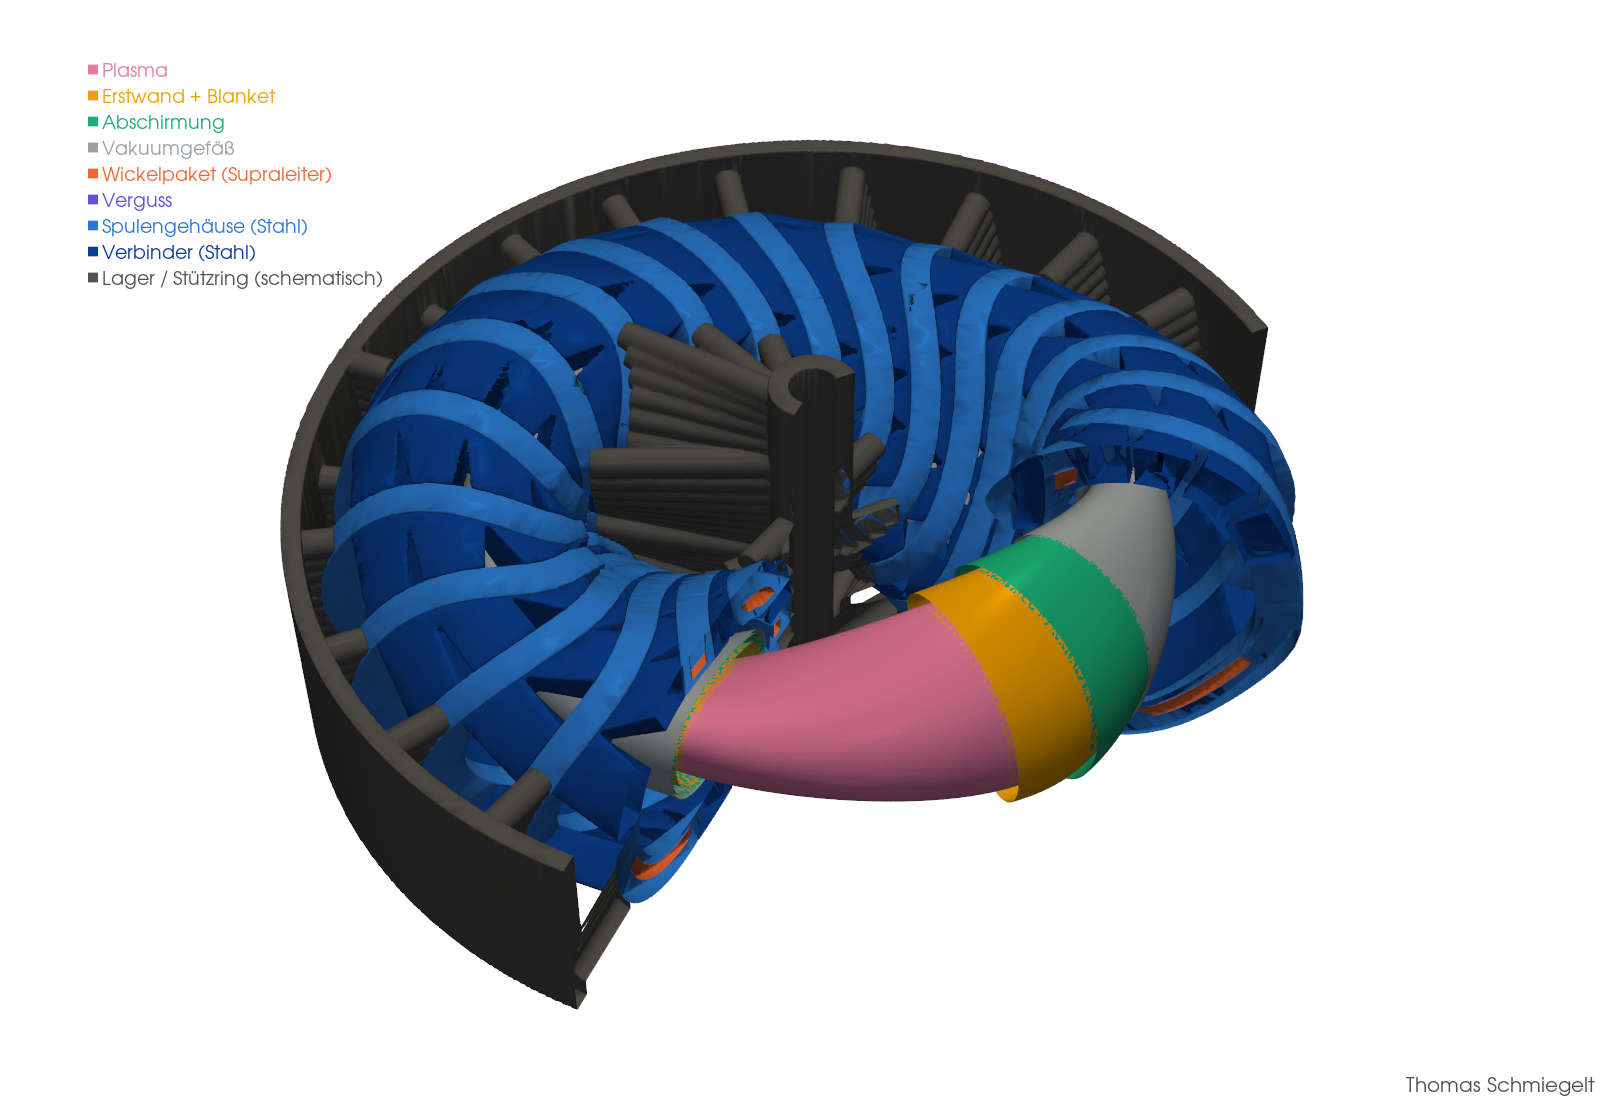
\includegraphics[width=\linewidth]{bilder/modell3d_V1_schnitt.png}\\\footnotesize PicoGK-Modell, Treppenschnitt\end{minipage}\hfill
\caption{Vorschlag V1 des Ersatzmodells}\end{figure}
\clearpage
\subsection{Tragwerksversuch E (dickste Wände)}\label{sb:E_test}
\noindent\textbf{Urteil: }Gleiche 16 Spulen wie der Ausgangsentwurf; nur das Tragwerk ist verändert.\par\smallskip
\begin{minipage}[t]{0.46\linewidth}\small\begin{tabular}[t]{@{}lr@{}}\toprule\multicolumn{2}{@{}l}{\textbf{Stellgrößen}}\\\midrule
Abstand Spule–Plasma & \num{0.180} \\
Spulen gesamt & 16 \\
Spulen je halbe Periode & \num{4} \\
Länge je Spule & \num{4.50} \\
Kraftziel & \num{0.000} \\
Wand innen & \num{0.60} \\
Seitenwand & \num{0.40} \\
Außenwand min. & \num{0.80} \\
Außenwand Zusatz & \num{0.60} \\
Verbindersteifigkeit & \num{200} \\
Verbinder je Paar & \num{12} \\
Lagerradius & \num{2.50} \\
\bottomrule\end{tabular}\end{minipage}\hfill
\begin{minipage}[t]{0.5\linewidth}\small\begin{tabular}[t]{@{}lr@{}}\toprule\multicolumn{2}{@{}l}{\textbf{Ergebnisse}}\\\midrule
$\sigma_{99}$ Stahl & \num{481} MPa \\
größtes Element & \num{2455} MPa \\
$P_m$ max. / 99 \% & \num{2396} / \num{736} MPa \\
$P_m+P_b$ max. & \num{2515} MPa \\
Verbinder σ99 & \num{276} MPa \\
Verformung max. & \num{41} mm \\
Dehnung Wickelpaket & \num{0.31} \% \\
Strom je Spule & \num{22.1} MA \\
Feld am Leiter & \num{18.7} T \\
Auslastung / Marge & \num{34} \% / \num{22} K \\
Feldfehler $B\cdot n$ & \num{2.71} ‰ \\
Freiraum Plasma–Gehäuse & \num{1.53} m \\
Kernheizung / Fluenz & \num{25} W/m³ / 2.1e17 \\
Stahl Gehäuse + Verbinder & \num{17.6} + \num{19.4} kt \\
Verbinder gebaut & 168 \\
\bottomrule\end{tabular}\end{minipage}\par\medskip
\begin{figure}[H]\centering
\begin{minipage}[t]{0.49\linewidth}\centering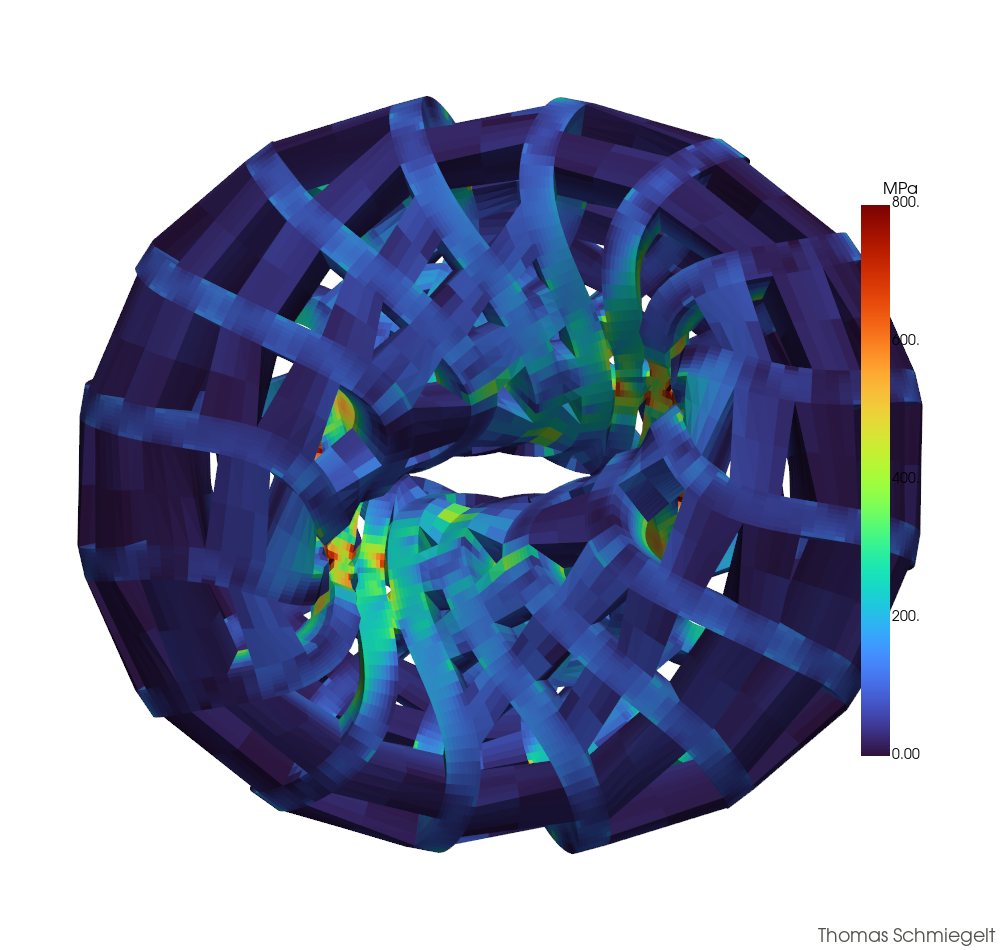
\includegraphics[width=\linewidth]{bilder/spannung_E_test.png}\\\footnotesize Vergleichsspannung im Stahl (Draufsicht, 0–800 MPa)\end{minipage}\hfill
\begin{minipage}[t]{0.49\linewidth}\centering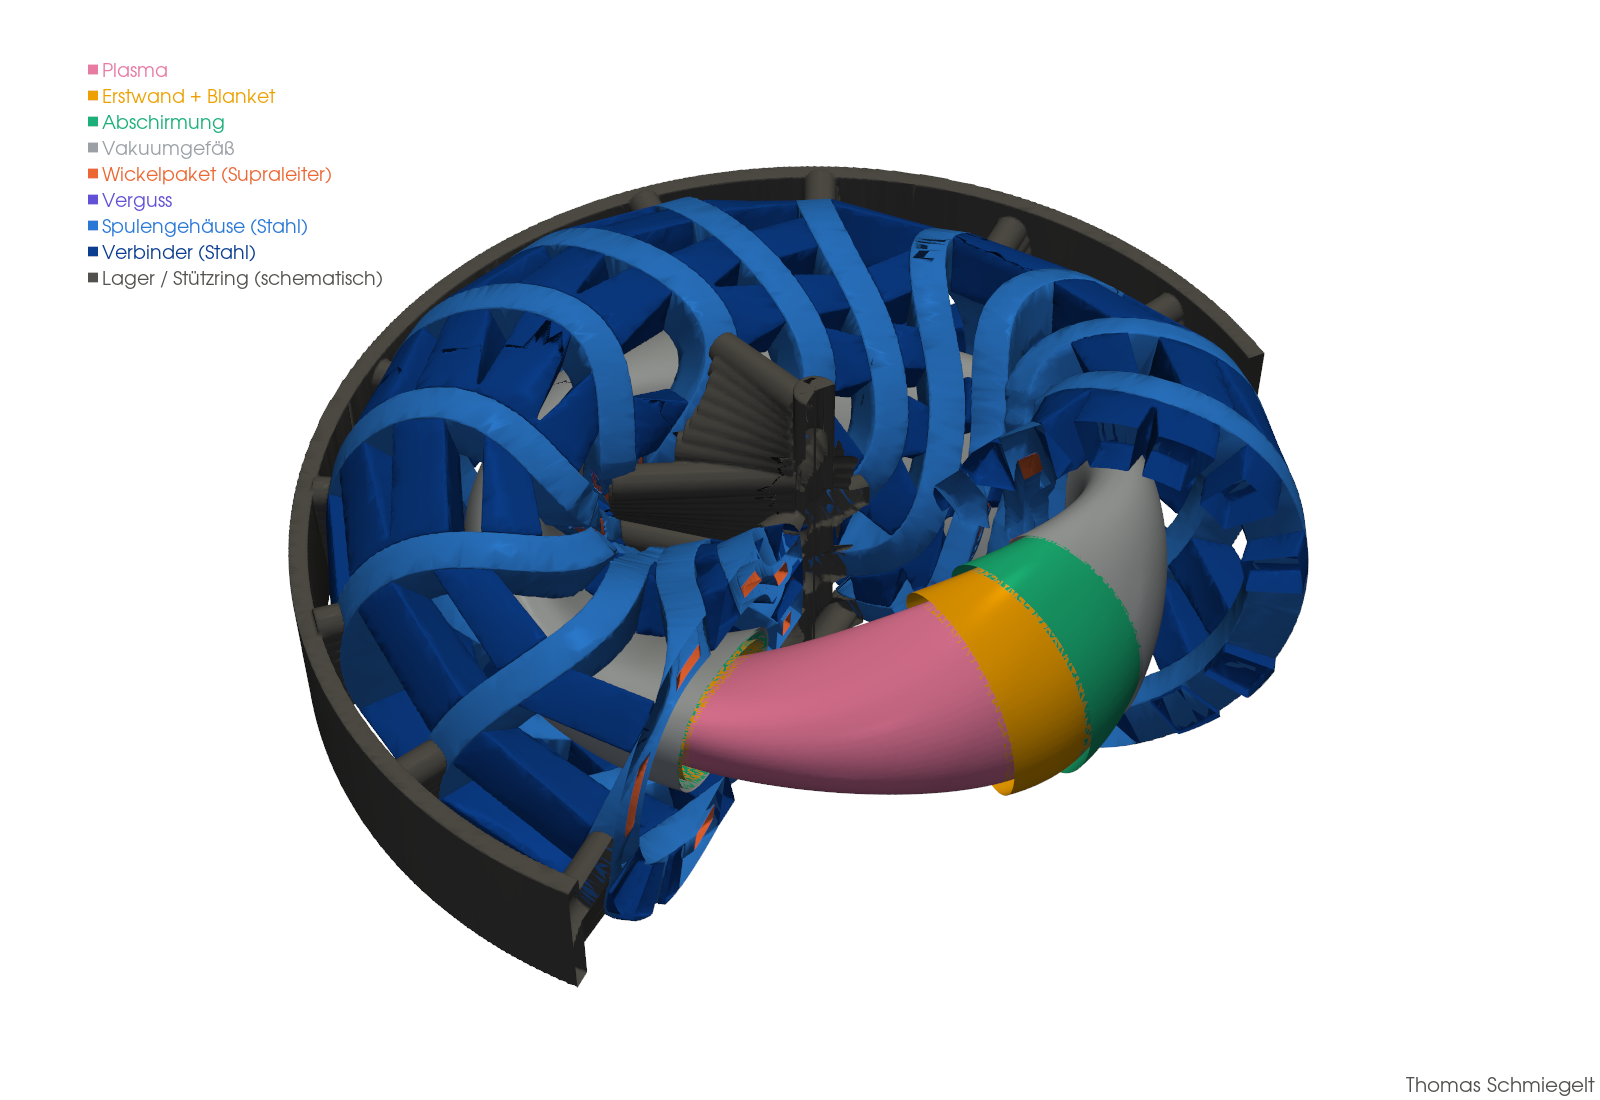
\includegraphics[width=\linewidth]{bilder/modell3d_E_test_schnitt.png}\\\footnotesize PicoGK-Modell, Treppenschnitt\end{minipage}\hfill
\caption{Tragwerksversuch E (dickste Wände)}\end{figure}
\clearpage
\subsection{Tragwerksversuch A (Ausgangsentwurf)}\label{sb:A_test}
\noindent\textbf{Urteil: }Gleiche 16 Spulen wie der Ausgangsentwurf; nur das Tragwerk ist verändert.\par\smallskip
\begin{minipage}[t]{0.46\linewidth}\small\begin{tabular}[t]{@{}lr@{}}\toprule\multicolumn{2}{@{}l}{\textbf{Stellgrößen}}\\\midrule
Abstand Spule–Plasma & \num{0.180} \\
Spulen gesamt & 16 \\
Spulen je halbe Periode & \num{4} \\
Länge je Spule & \num{4.50} \\
Kraftziel & \num{0.000} \\
Wand innen & \num{0.35} \\
Seitenwand & \num{0.24} \\
Außenwand min. & \num{0.45} \\
Außenwand Zusatz & \num{0.30} \\
Verbindersteifigkeit & \num{50} \\
Verbinder je Paar & \num{6} \\
Lagerradius & \num{2.50} \\
\bottomrule\end{tabular}\end{minipage}\hfill
\begin{minipage}[t]{0.5\linewidth}\small\begin{tabular}[t]{@{}lr@{}}\toprule\multicolumn{2}{@{}l}{\textbf{Ergebnisse}}\\\midrule
$\sigma_{99}$ Stahl & \num{2129} MPa \\
größtes Element & \num{8454} MPa \\
Verbinder σ99 & \num{675} MPa \\
Verformung max. & \num{399} mm \\
Dehnung Wickelpaket & \num{0.76} \% \\
Strom je Spule & \num{22.1} MA \\
Feld am Leiter & \num{18.7} T \\
Auslastung / Marge & \num{34} \% / \num{22} K \\
Feldfehler $B\cdot n$ & \num{2.71} ‰ \\
Freiraum Plasma–Gehäuse & \num{1.77} m \\
Kernheizung / Fluenz & \num{2} W/m³ / 1.8e16 \\
Stahl Gehäuse + Verbinder & \num{8.5} + \num{7.0} kt \\
Verbinder gebaut & 90 \\
\bottomrule\end{tabular}\end{minipage}\par\medskip
\begin{figure}[H]\centering
\begin{minipage}[t]{0.49\linewidth}\centering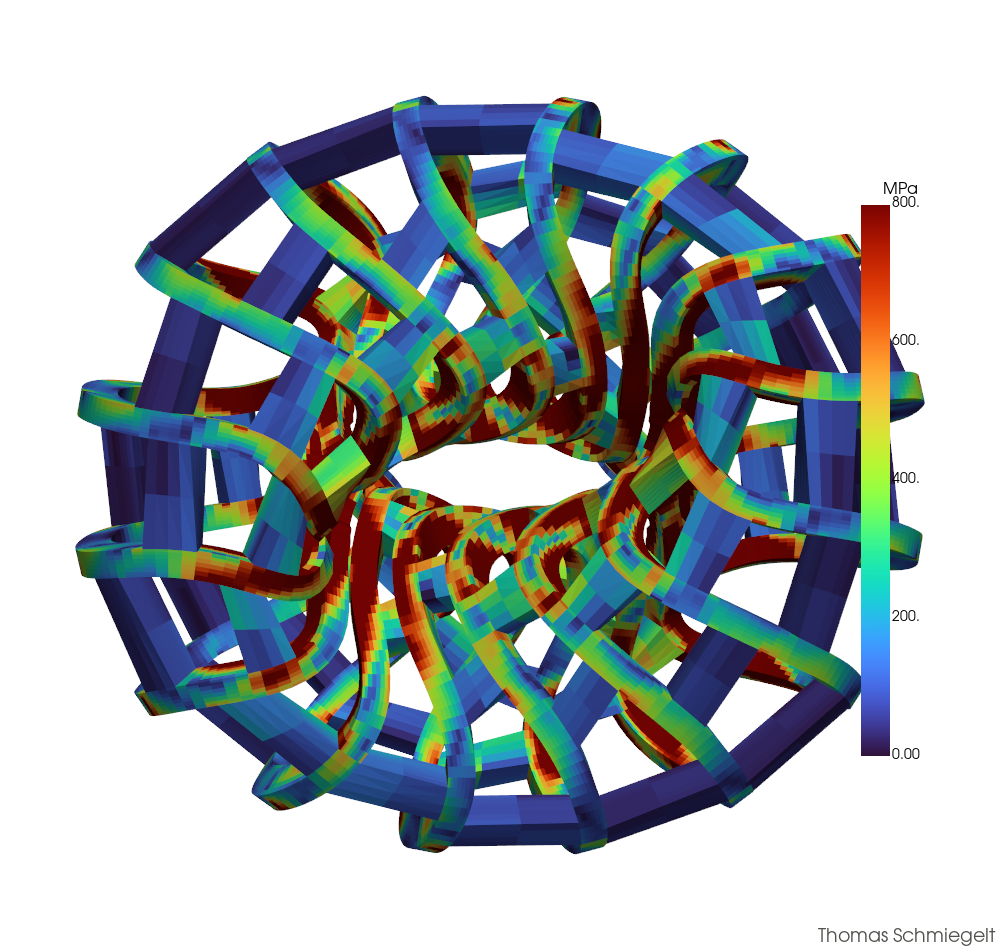
\includegraphics[width=\linewidth]{bilder/spannung_A_test.png}\\\footnotesize Vergleichsspannung im Stahl (Draufsicht, 0–800 MPa)\end{minipage}\hfill
\begin{minipage}[t]{0.49\linewidth}\centering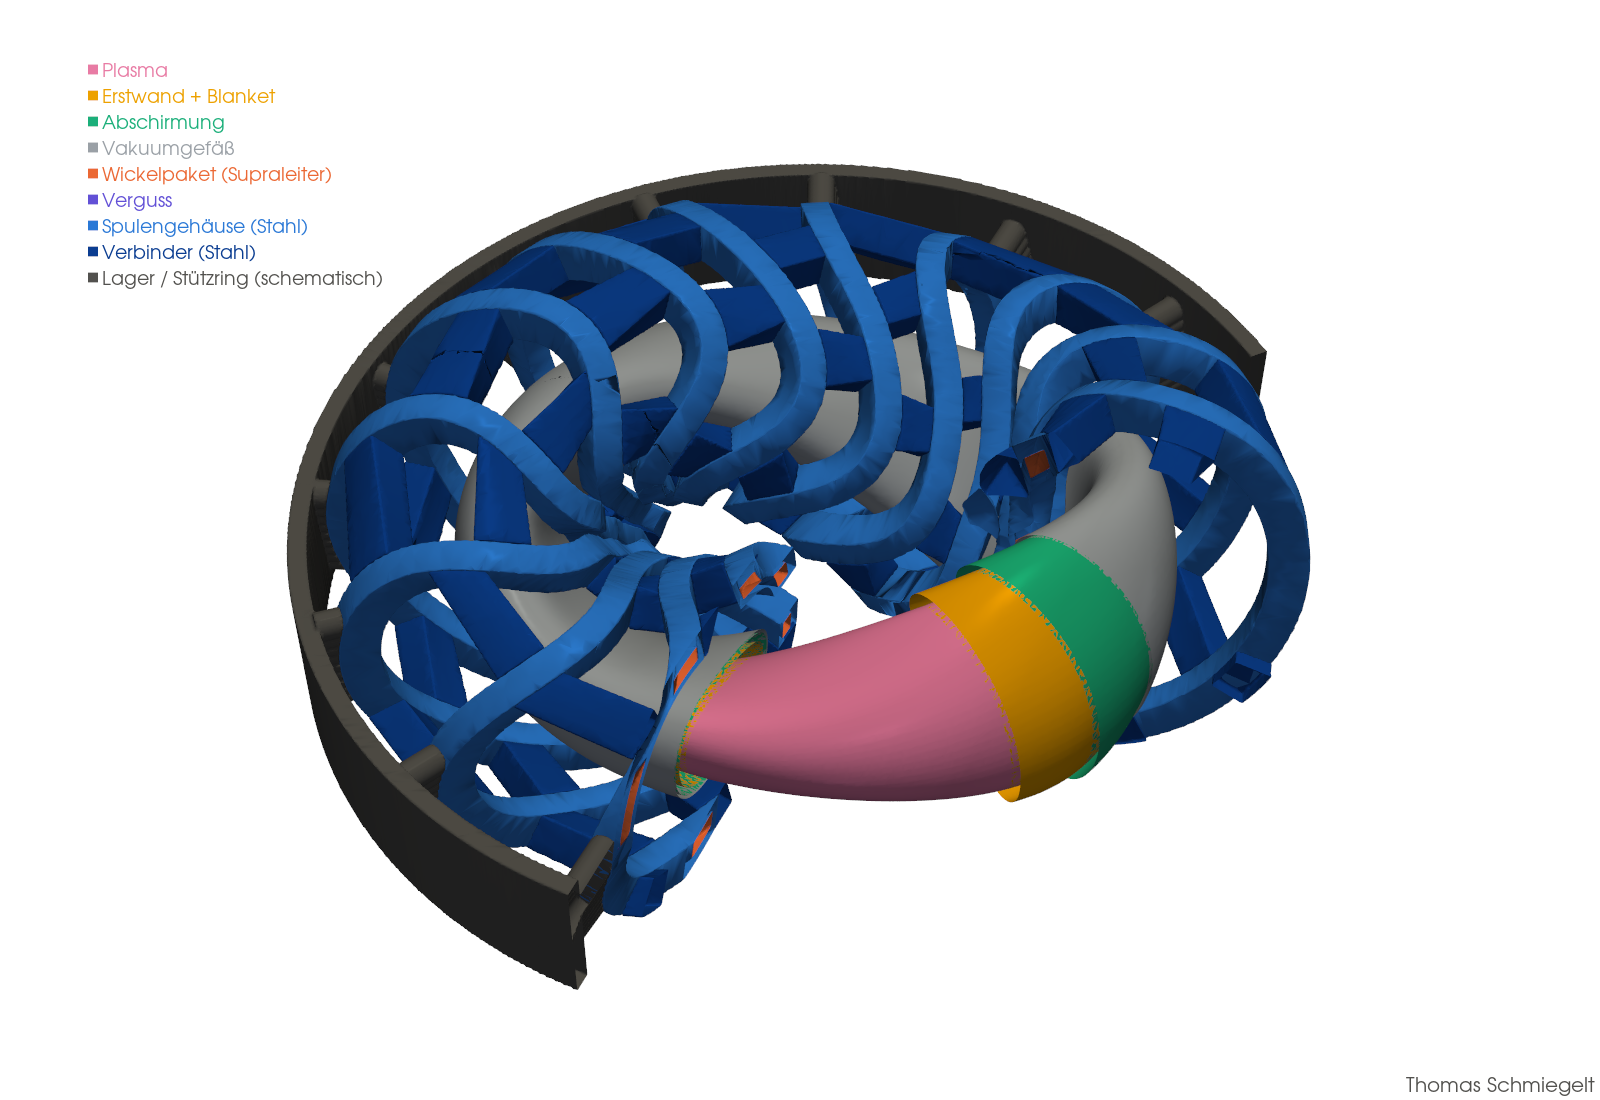
\includegraphics[width=\linewidth]{bilder/modell3d_A_test_schnitt.png}\\\footnotesize PicoGK-Modell, Treppenschnitt\end{minipage}\hfill
\caption{Tragwerksversuch A (Ausgangsentwurf)}\end{figure}
